\documentclass[../Matt_Gebert_Honours_Thesis.tex]{subfiles}

\begin{document}
% The results to here will be compared alongside data after stamping the same devices with thin oxides in  \cref{chap:thinoxidegraphene}.

	In this chapter, I explore various liquid metal printing techniques\cite{zavabeti_liquid_2017} that were further developed through my work to transfer oxides on a graphene device. Progress towards successful oxide transfer was achieved by using many dummy devices consisting of gold pads but no device. The use of liquid metal to deposit thin oxides has been named as printing, and in this chapter I'll refer to two methods that allow this printing, namely stamping and smearing.
	
	During this time I worked closely with Kourosh Kalantar-zadeh's group at RMIT (Royal Melbourne institute of technology), in particular Ali Zavabeti, Torben Daeneke, Nitu Syed, Hareem Khan and Paul Atkin in developing this work.

	\section{Stamping}\label{sec:printing}
		The traditional technique of mechanical exfoliation is at the core creating many new materials in current research. This is also the case with the liquid metal printing technique. In this section, I will discuss \aluminimumoxide{}, \tinoxide{} and \bismuthoxide{}, all of which are synthesised by `stamping' onto liquid metal droplets.
		
	\subsection{Al$_2$O$_3$}
		Aluminium oxide was the first oxide Ali and I investigated for use in our devices. This was for the reason that generally \aluminimumoxide{} is very easy to make by grinding up aluminium wire. I have already detailed the bare process in \cref{sec:oxidestamp_chap2}. An example of the droplets created using the mortar and pestle is seen in \cref{fig:al_synthesis}, and the touching process.		
		\begin{figure}[H]
			\centering
			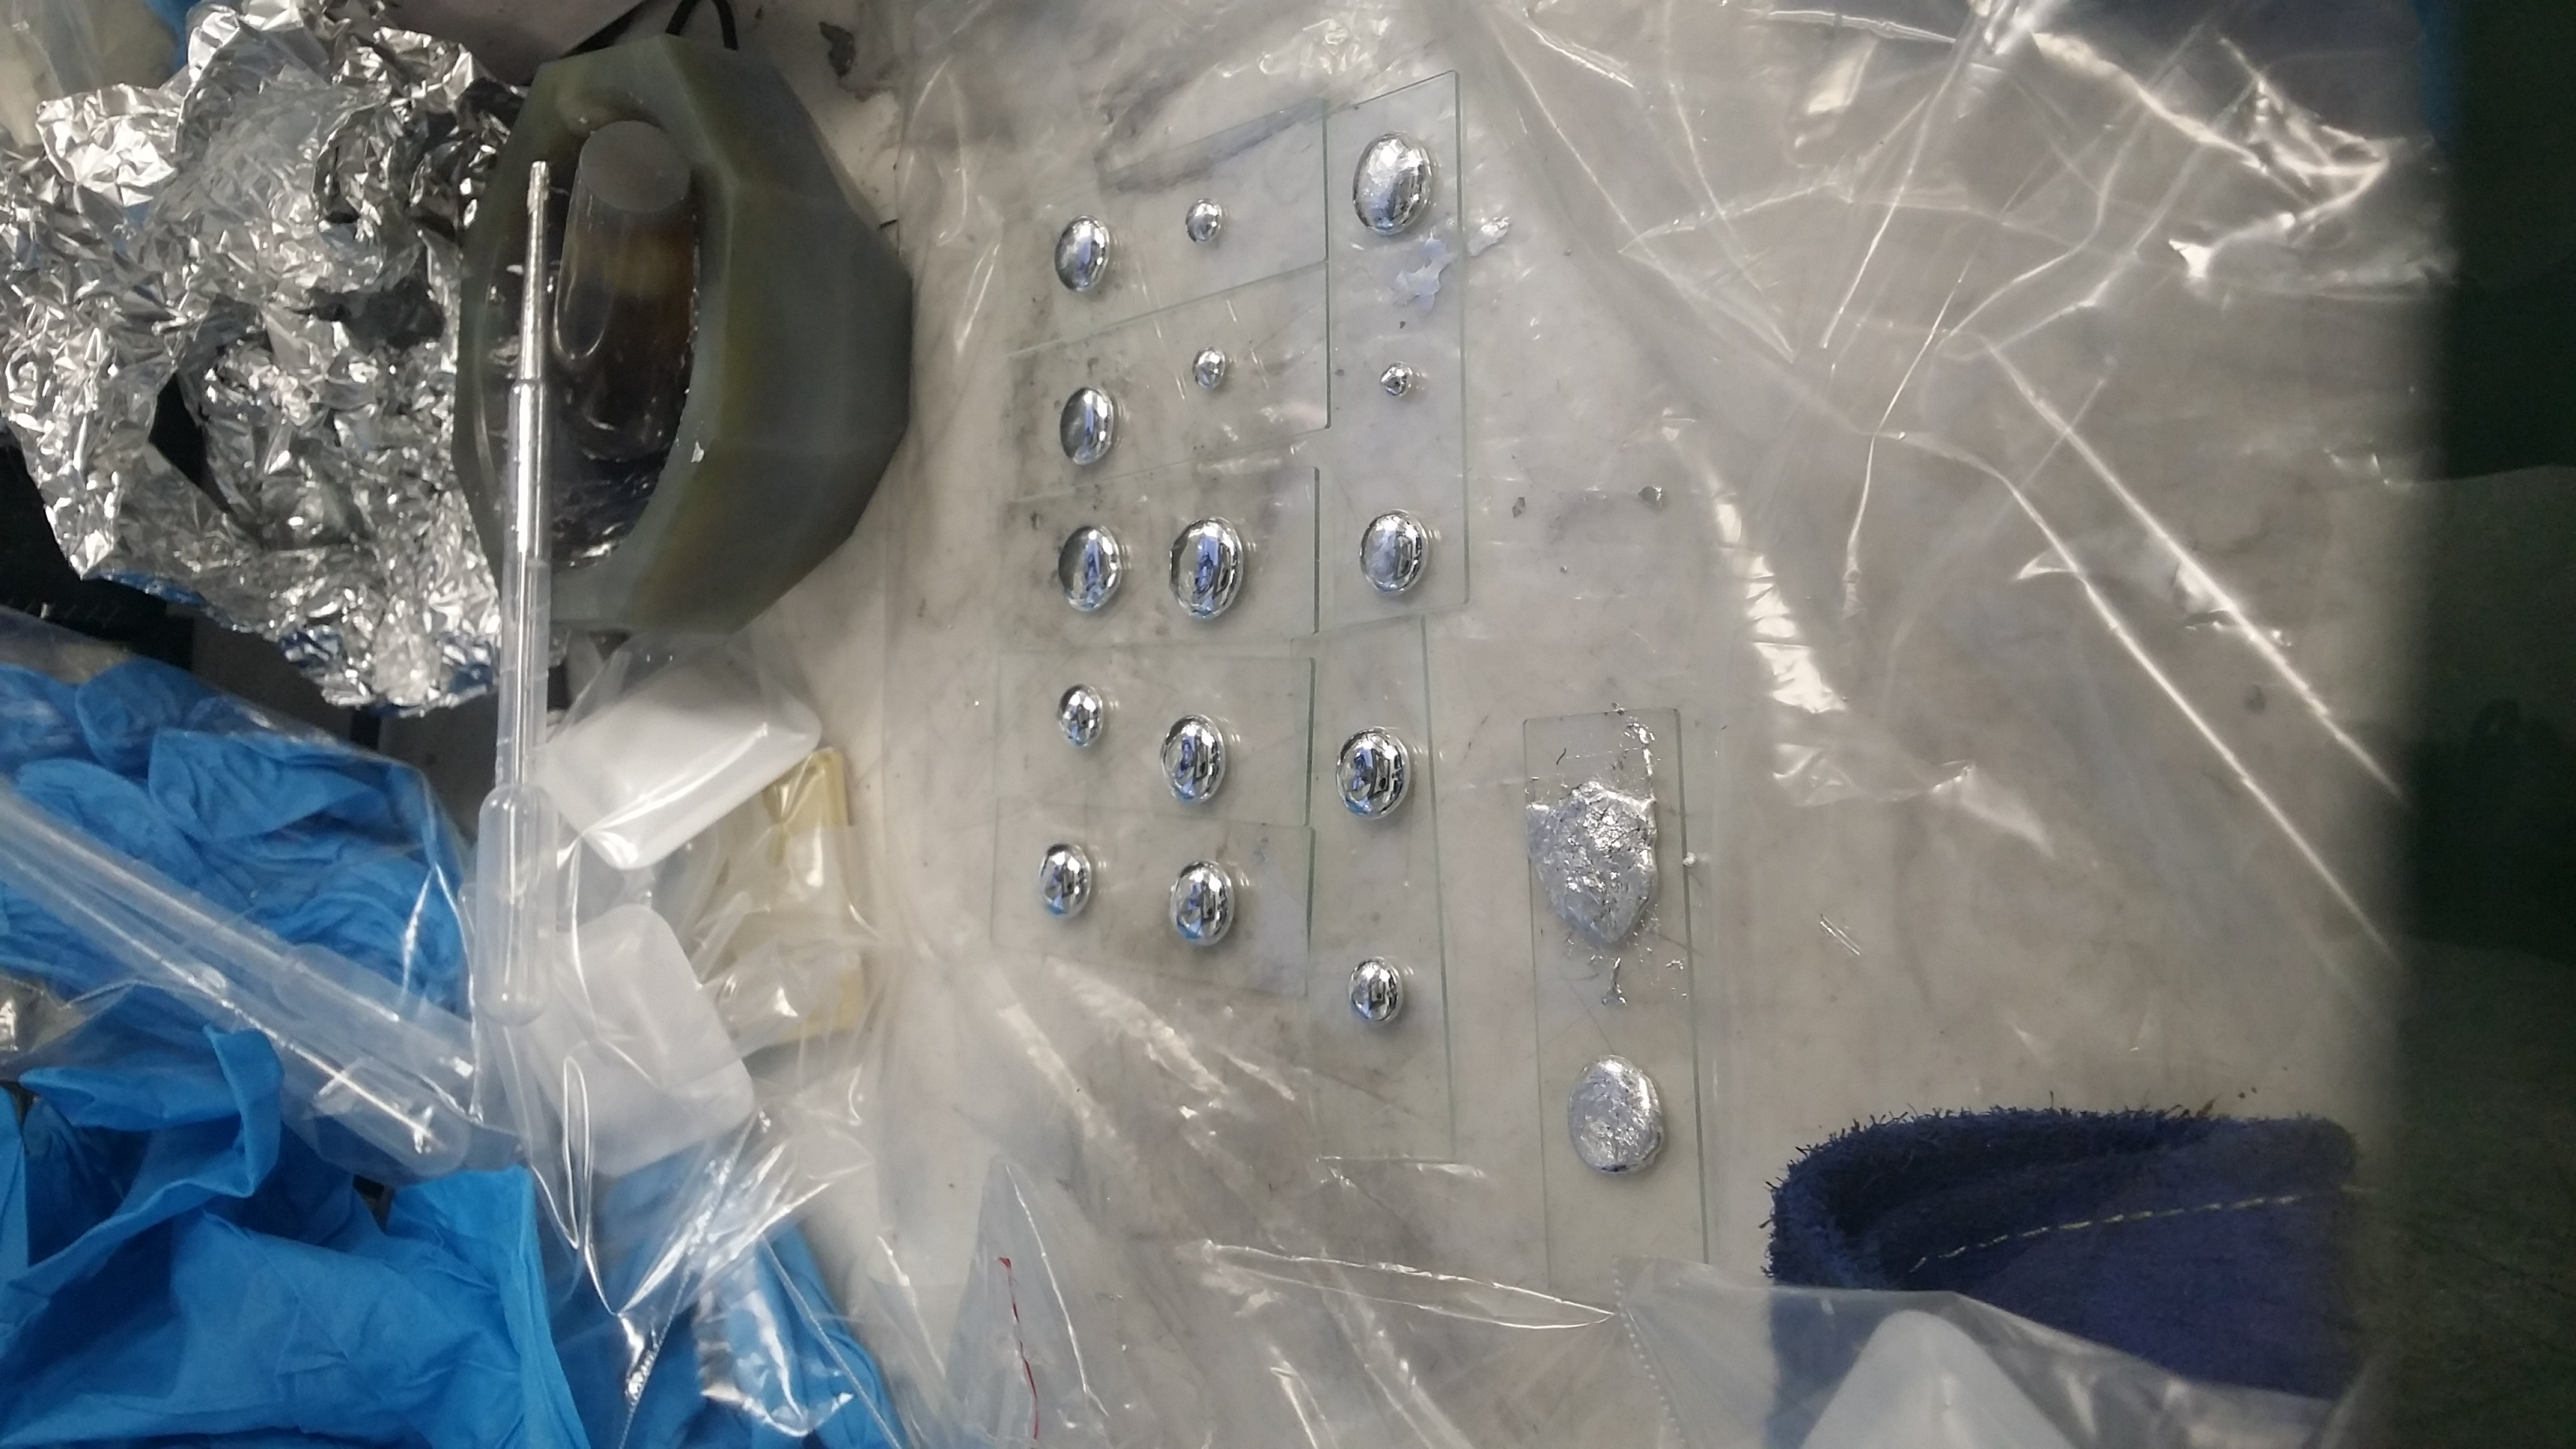
\includegraphics[width=0.3\textwidth,angle=270]{chap5/al2o3/setup}
			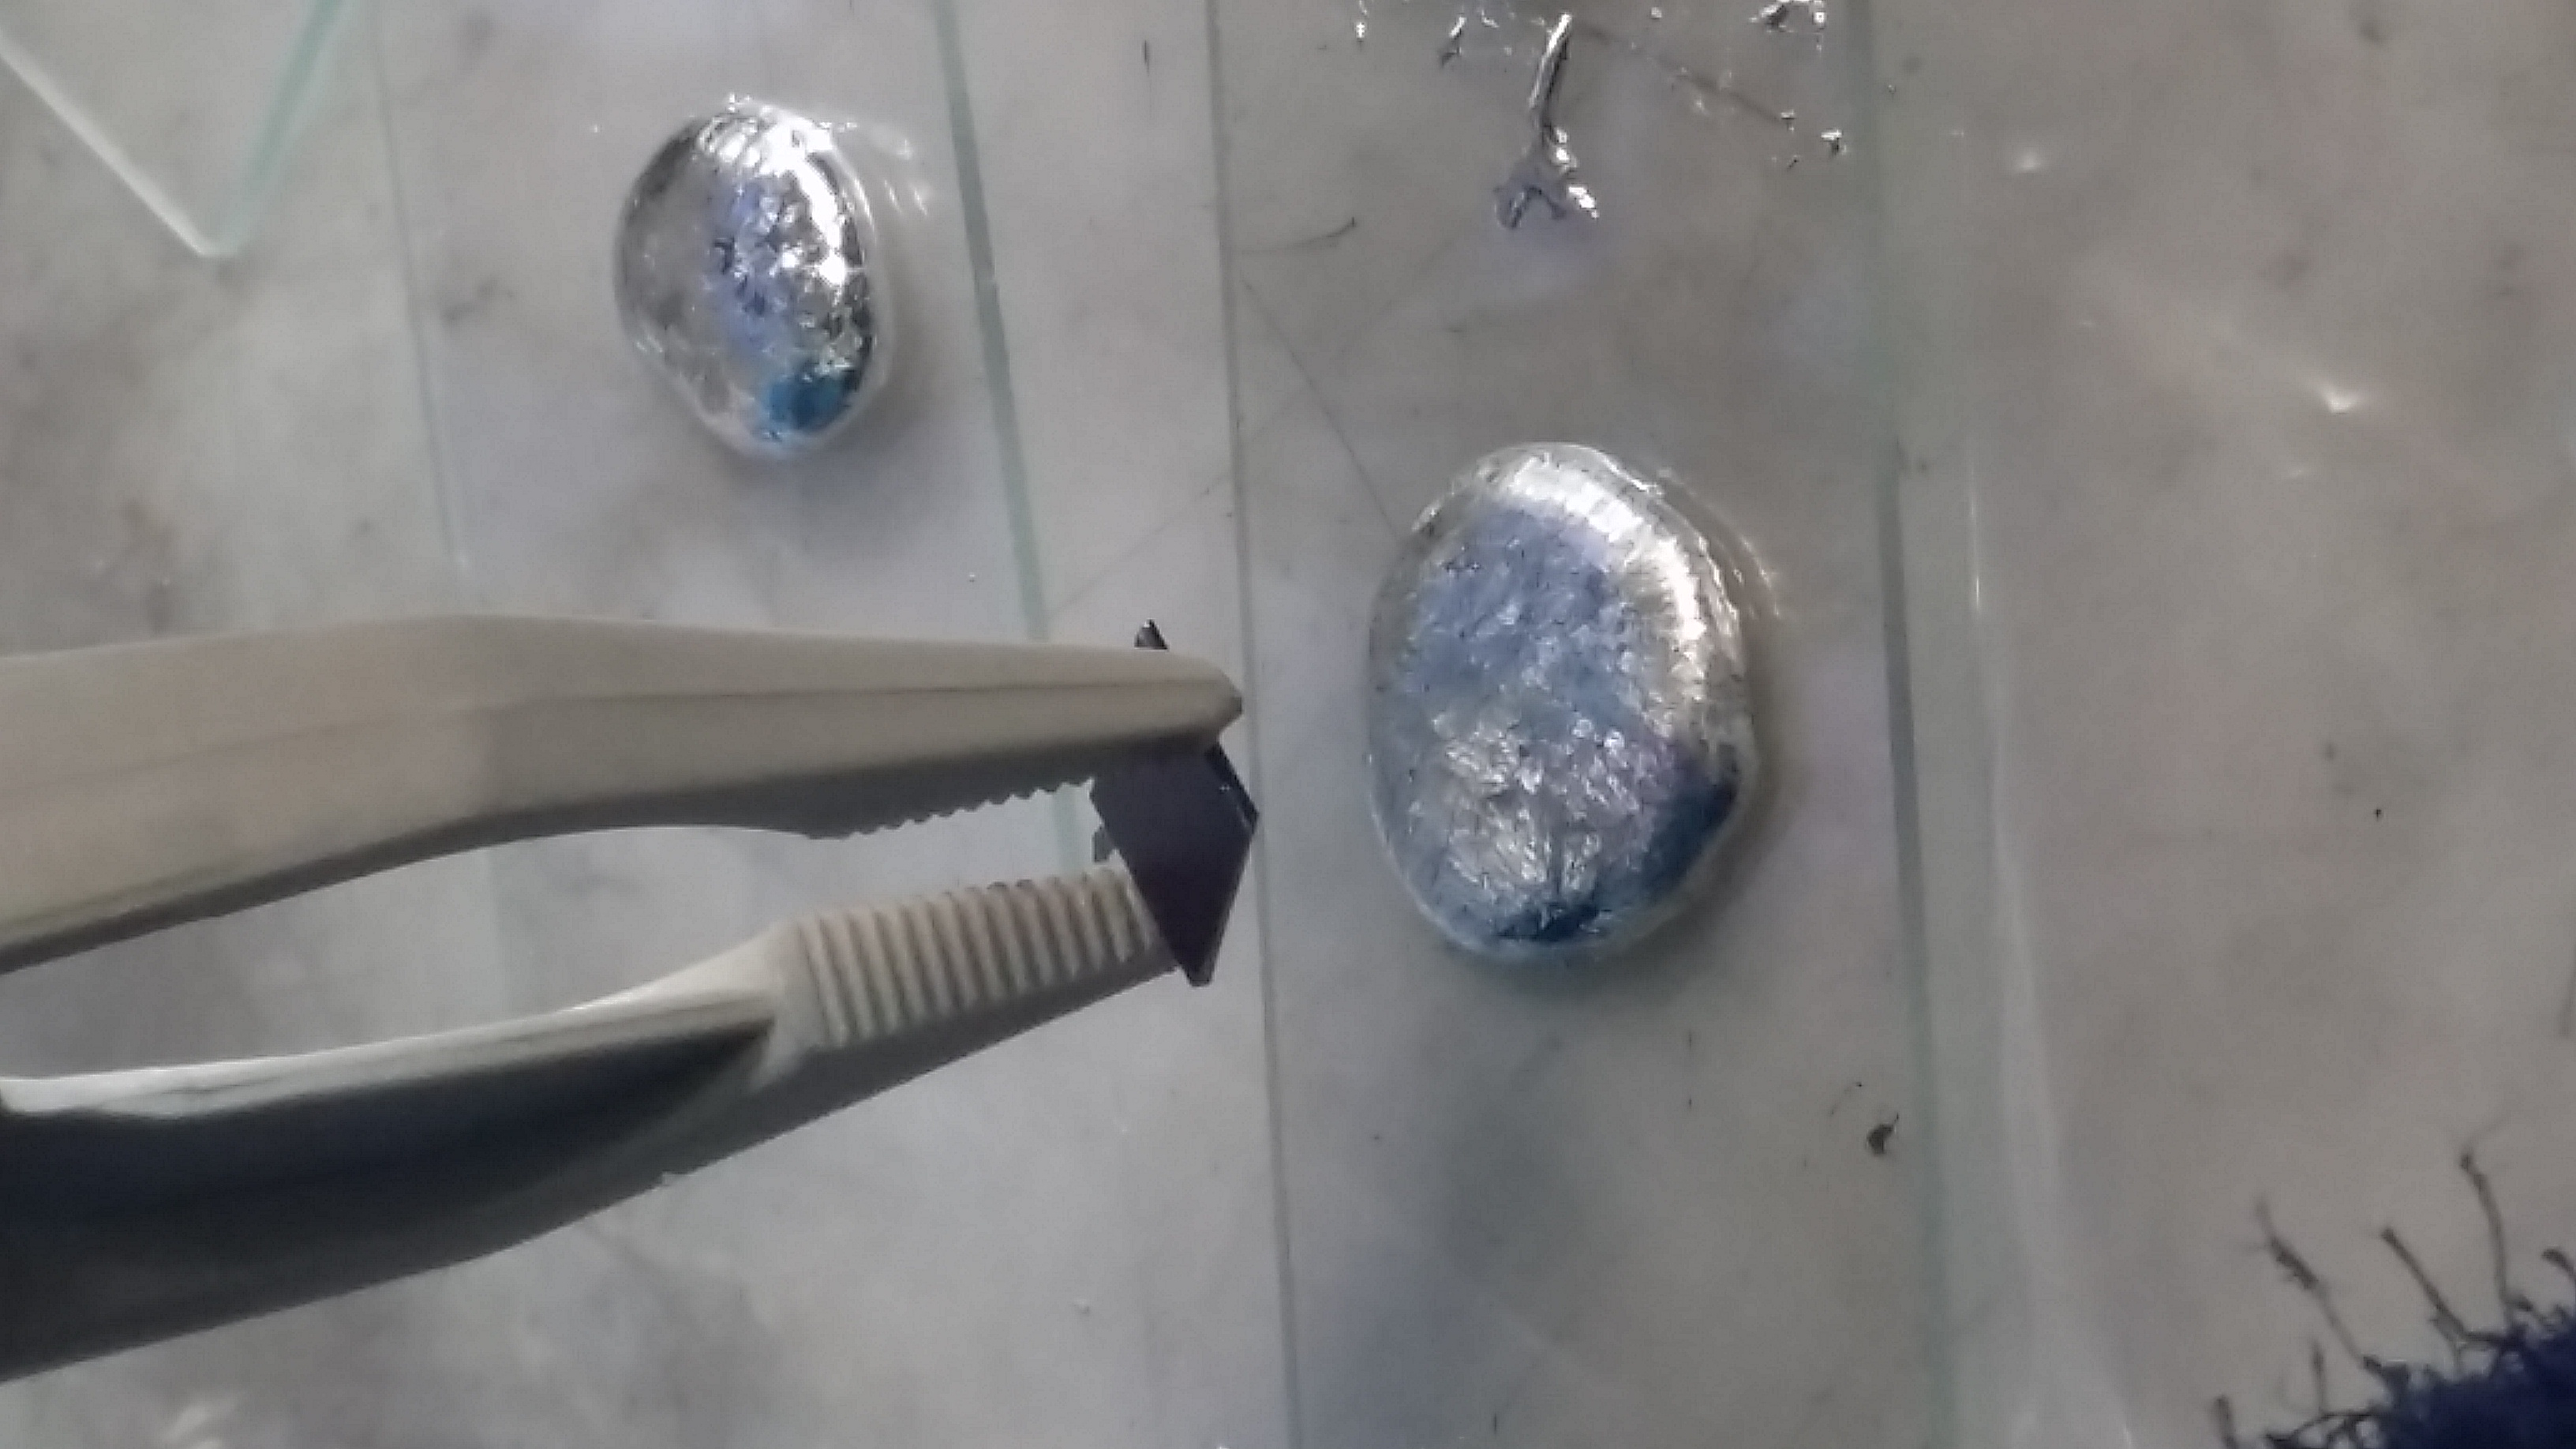
\includegraphics[width=0.3\textwidth,angle=270]{chap5/al2o3/stamp}
			\caption[\aluminimumoxide{} synthesis process]{Synthesis process for printing \aluminimumoxide{} }\label{fig:al_synthesis}
		\end{figure}
		We tested over 30 samples on droplets, varying radii and exposure time to air (to let the oxide form on the surface). Unfortunately very little material transferred in any of these tests, with only one clean deposition as shown in \cref{fig:al2o3_1}. 
		\begin{figure}[H]
			\begin{subfigure}[t]{0.5\textwidth}
				\centering
				\includegraphics[width=0.85\textwidth,angle=0]{chap5/al2o3/transfer1}
				\caption{\aluminimumoxide{} on \silicondioxide{} (unknown thickness).}\label{fig:al2o3_1}
			\end{subfigure}
			\begin{subfigure}[t]{0.5\textwidth}
				\centering
				\includegraphics[width=0.85\textwidth,angle=0]{chap5/al2o3/transfer2}
				\caption{Non uniform oxide deposition, but some thin areas}\label{fig:al2o3_2}
			\end{subfigure}
			\begin{subfigure}[t]{0.5\textwidth}
				\centering
				\includegraphics[width=0.85\textwidth,angle=0]{chap5/al2o3/transfer3}
				\caption{Metal residue left after an unsuccessful transfer}\label{fig:al2o3_3}
			\end{subfigure}
			\begin{subfigure}[t]{0.5\textwidth}
				\centering
				\includegraphics[width=0.85\textwidth,angle=0]{chap5/al2o3/transfer4}
				\caption{Metal remaining, with traces of thick (gallium) oxide}\label{fig:al2o3_4}
			\end{subfigure}
		\caption[\aluminimumoxide{} printing on \silicondioxide{}]{Deposition of \aluminimumoxide{} onto \silicondioxide{}. Scale bar: 0.13mm}\label{fig:transfer_al_on_si}
		\end{figure}
		More commonly than not though, the liquid metal begun interacting with gold pads and adhering through any oxide layer, or no oxide was deposited (\cref{fig:transfer_al_on_au&si})
		\begin{figure}[H]
			\begin{subfigure}[t]{0.5\textwidth}
				\centering
				\includegraphics[width=0.85\textwidth,angle=0]{chap5/al2o3/gtransfer1}
				\caption{Adhesion of gallium to gold pads}\label{fig:al2o3_g1}
			\end{subfigure}
			\begin{subfigure}[t]{0.5\textwidth}
				\centering
				\includegraphics[width=0.85\textwidth,angle=0]{chap5/al2o3/gtransfer2}
				\caption{After cleaning off gallium, remains of gold pads}\label{fig:al2o3_g2}
			\end{subfigure}
		\end{figure}
		\begin{figure}[H]
			\ContinuedFloat
			\begin{subfigure}[t]{0.5\textwidth}
				\centering
				\includegraphics[width=0.85\textwidth,angle=0]{chap5/al2o3/gtransfer3}
				\caption{No oxide deposition, but surface contamination}\label{fig:al2o3_g3}
			\end{subfigure}
			\begin{subfigure}[t]{0.5\textwidth}
				\centering
				\includegraphics[width=0.85\textwidth,angle=0]{chap5/al2o3/gtransfer4}
				\caption{Gallium metal and some gallium oxide deposition}\label{fig:al2o3_g4}
			\end{subfigure}
			\caption[\aluminimumoxide{} printing onto Au on \silicondioxide{}]{Deposition of \aluminimumoxide{} onto Au on \silicondioxide{}}\label{fig:transfer_al_on_au&si}
		\end{figure}
		We also attempted spreading oxide on transferred CVD graphene, but no evidence of oxide transfer was found optically (\cref{fig:transfer_al_on_cvd}).
		\begin{figure}[H]
			\begin{subfigure}[t]{0.5\textwidth}
				\centering
				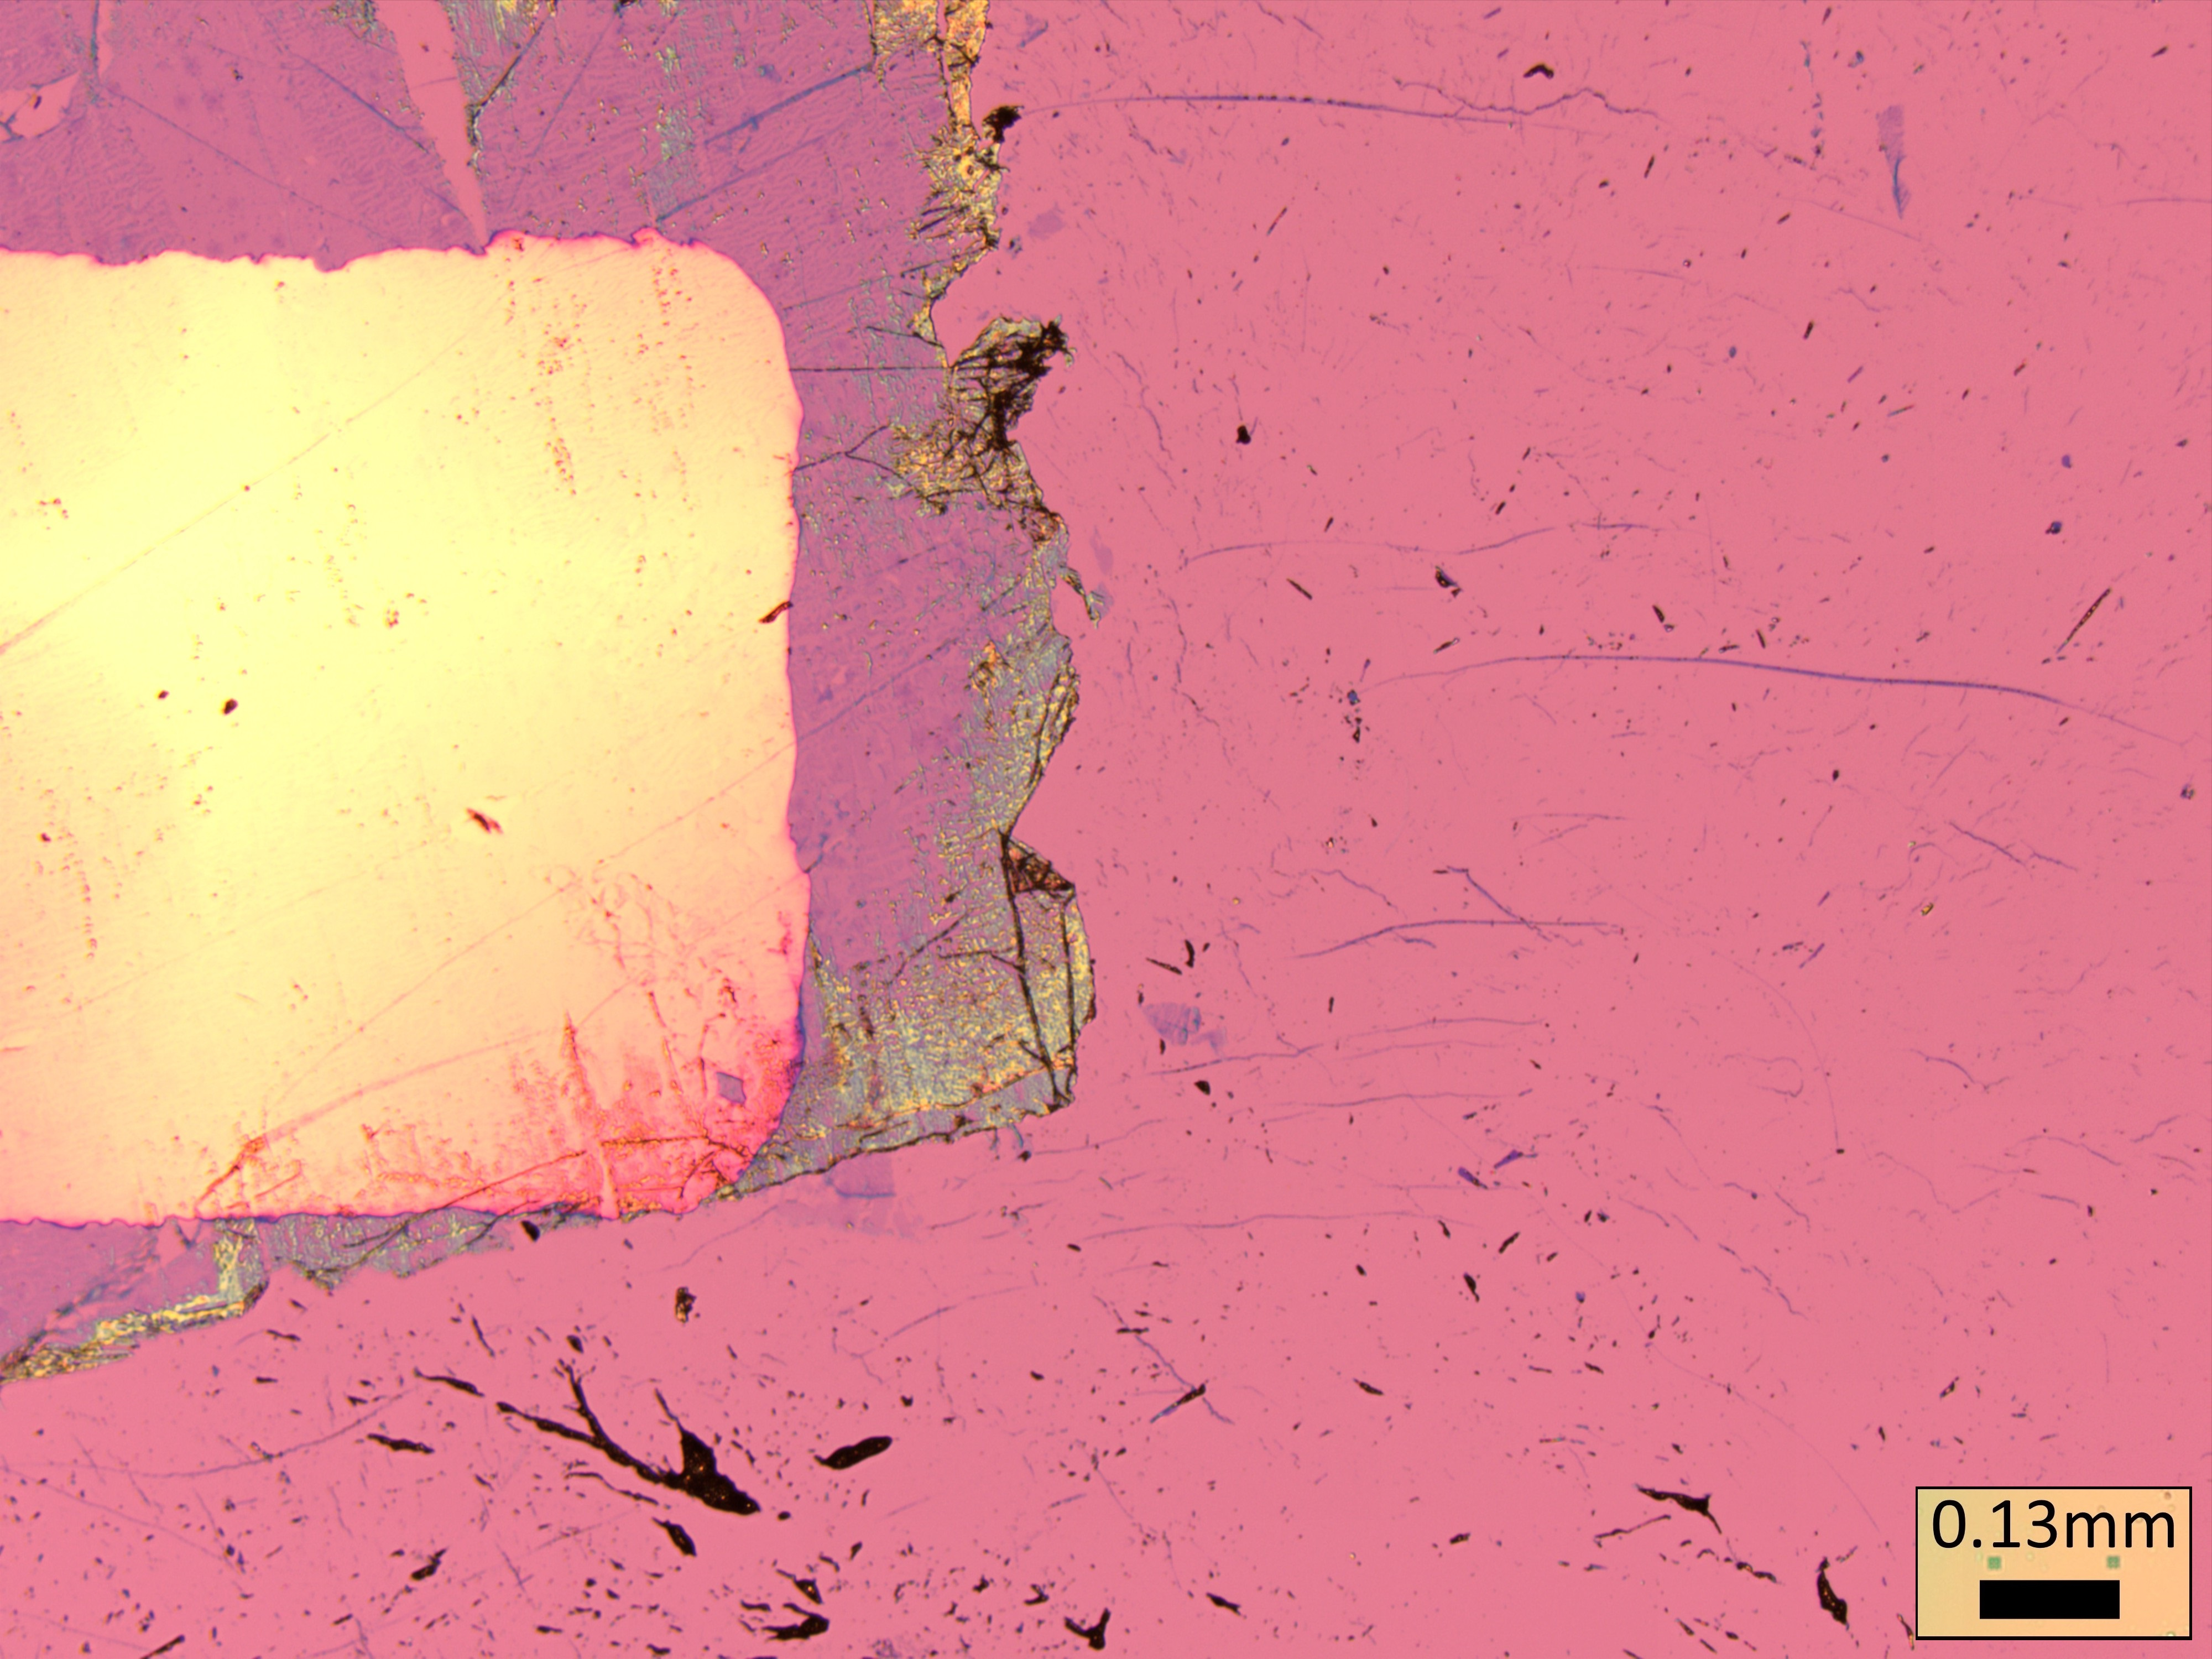
\includegraphics[width=0.85\textwidth,angle=0]{chap5/al2o3/ctransfer1}
				\caption{}\label{fig:al2o3_c1}
			\end{subfigure}
			\begin{subfigure}[t]{0.5\textwidth}
				\centering
				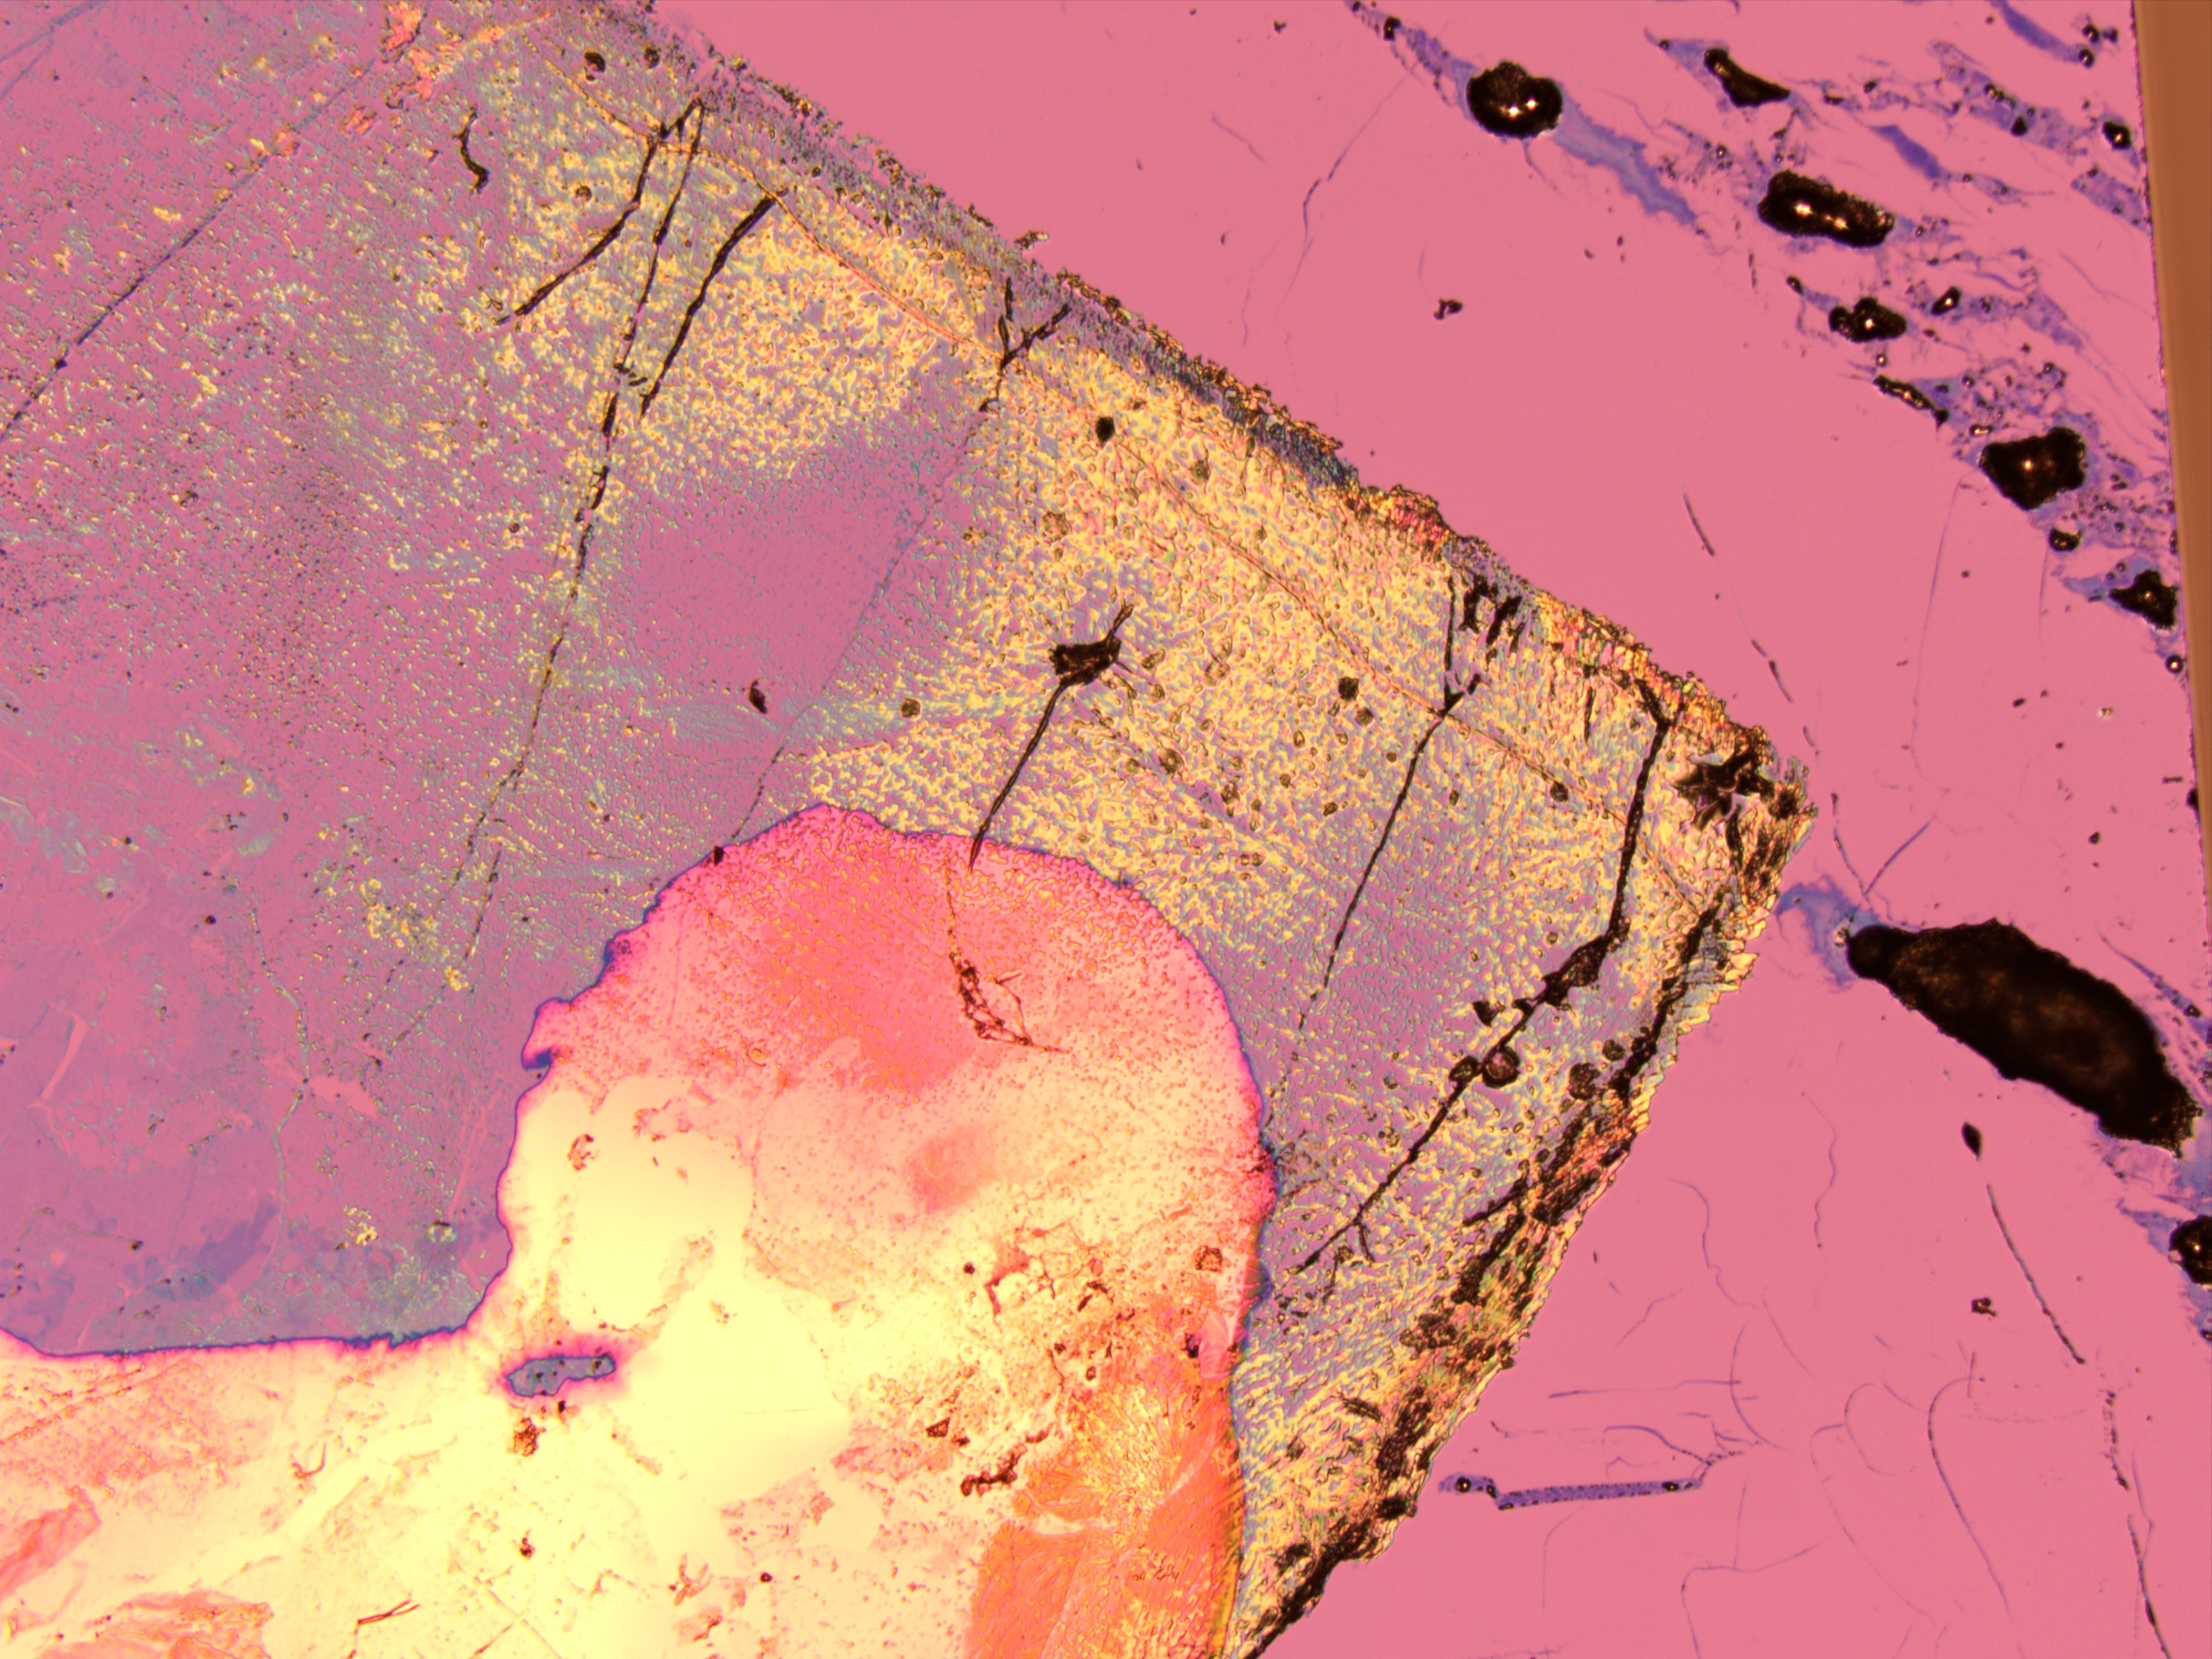
\includegraphics[width=0.85\textwidth,angle=0]{chap5/al2o3/ctransfer2}
				\caption{}\label{fig:al2o3_c2}
			\end{subfigure}
			\caption[\aluminimumoxide{} printing on CVD graphene \& \silicondioxide{}]{Contamination of CVD graphene without transfer of \aluminimumoxide{}.}\label{fig:transfer_al_on_cvd}
		\end{figure}
		After three trials using aluminium oxide and varying the exfoliation method, Torben suggested we try some other oxides for something more reliable and clean, particularly for the time window of this project. 
	
	\subsection{SnO \& Bi$_2$O$_3$}
	After switching from \aluminimumoxide{}, I tried to start using \tinoxide{}, \bismuthoxide{} and \galliumoxide{}(see \cref{sec:smearing} below). Hareem assisted me with transferring \bismuthoxide{} and \tinoxide{} onto desired substrates, using the same base method of exfoliation in a low oxygen fumehood, but with a few modifications. 
	
	Different from \aluminimumoxide{}, we used pure tin and bismuth (no need for a gallium alloy) and melted the chunks on a hotplate at 330 $^\circ$C and 270 $^\circ$C  respectively. We also used glass slides to `sacrifice' a layer of outer material before proceeding to attempt to exfoliate a layer of material.
	
	We had immediate success with this method for depositing onto bare substrates, as seen in \cref{fig:transfer_bi&sno_on_si}.
	\begin{figure}[H]
		\begin{subfigure}[t]{0.24\textwidth}
			\centering
			\includegraphics[width=0.95\textwidth,angle=0]{chap5/bi2o3/transfer1}
			\caption{Clean \bismuthoxide{} sheet - 5x}\label{fig:bi2o3_1}
		\end{subfigure}
		\begin{subfigure}[t]{0.24\textwidth}
			\centering
			\includegraphics[width=0.95\textwidth,angle=0]{chap5/bi2o3/transfer1_50x}
			\caption{Clean \bismuthoxide{} sheet - 50x}\label{fig:bi2o3_2}
		\end{subfigure}
		\begin{subfigure}[t]{0.24\textwidth}
			\centering
			\includegraphics[width=0.95\textwidth,angle=0]{chap5/sno/transfer1}
			\caption[\tinoxide{} transfer on \silicondioxide{}]{A clean transfer of \tinoxide{} onto \silicondioxide{} 5x}\label{fig:sno_1}
		\end{subfigure}
		\begin{subfigure}[t]{0.24\textwidth}
			\centering
			\includegraphics[width=0.95\textwidth,angle=0]{chap5/sno/transfer1_50x}
			\caption{Clean \tinoxide{} transfer 50x}\label{fig:sno_2}
		\end{subfigure}
		\begin{subfigure}[t]{0.24\textwidth}
			\centering
			\includegraphics[width=0.95\textwidth,angle=0]{chap5/bi2o3/transfer2}
			\caption{\bismuthoxide{} with nearby metal - 5x}\label{fig:bi2o3_3}
		\end{subfigure}
		\begin{subfigure}[t]{0.24\textwidth}
			\centering
			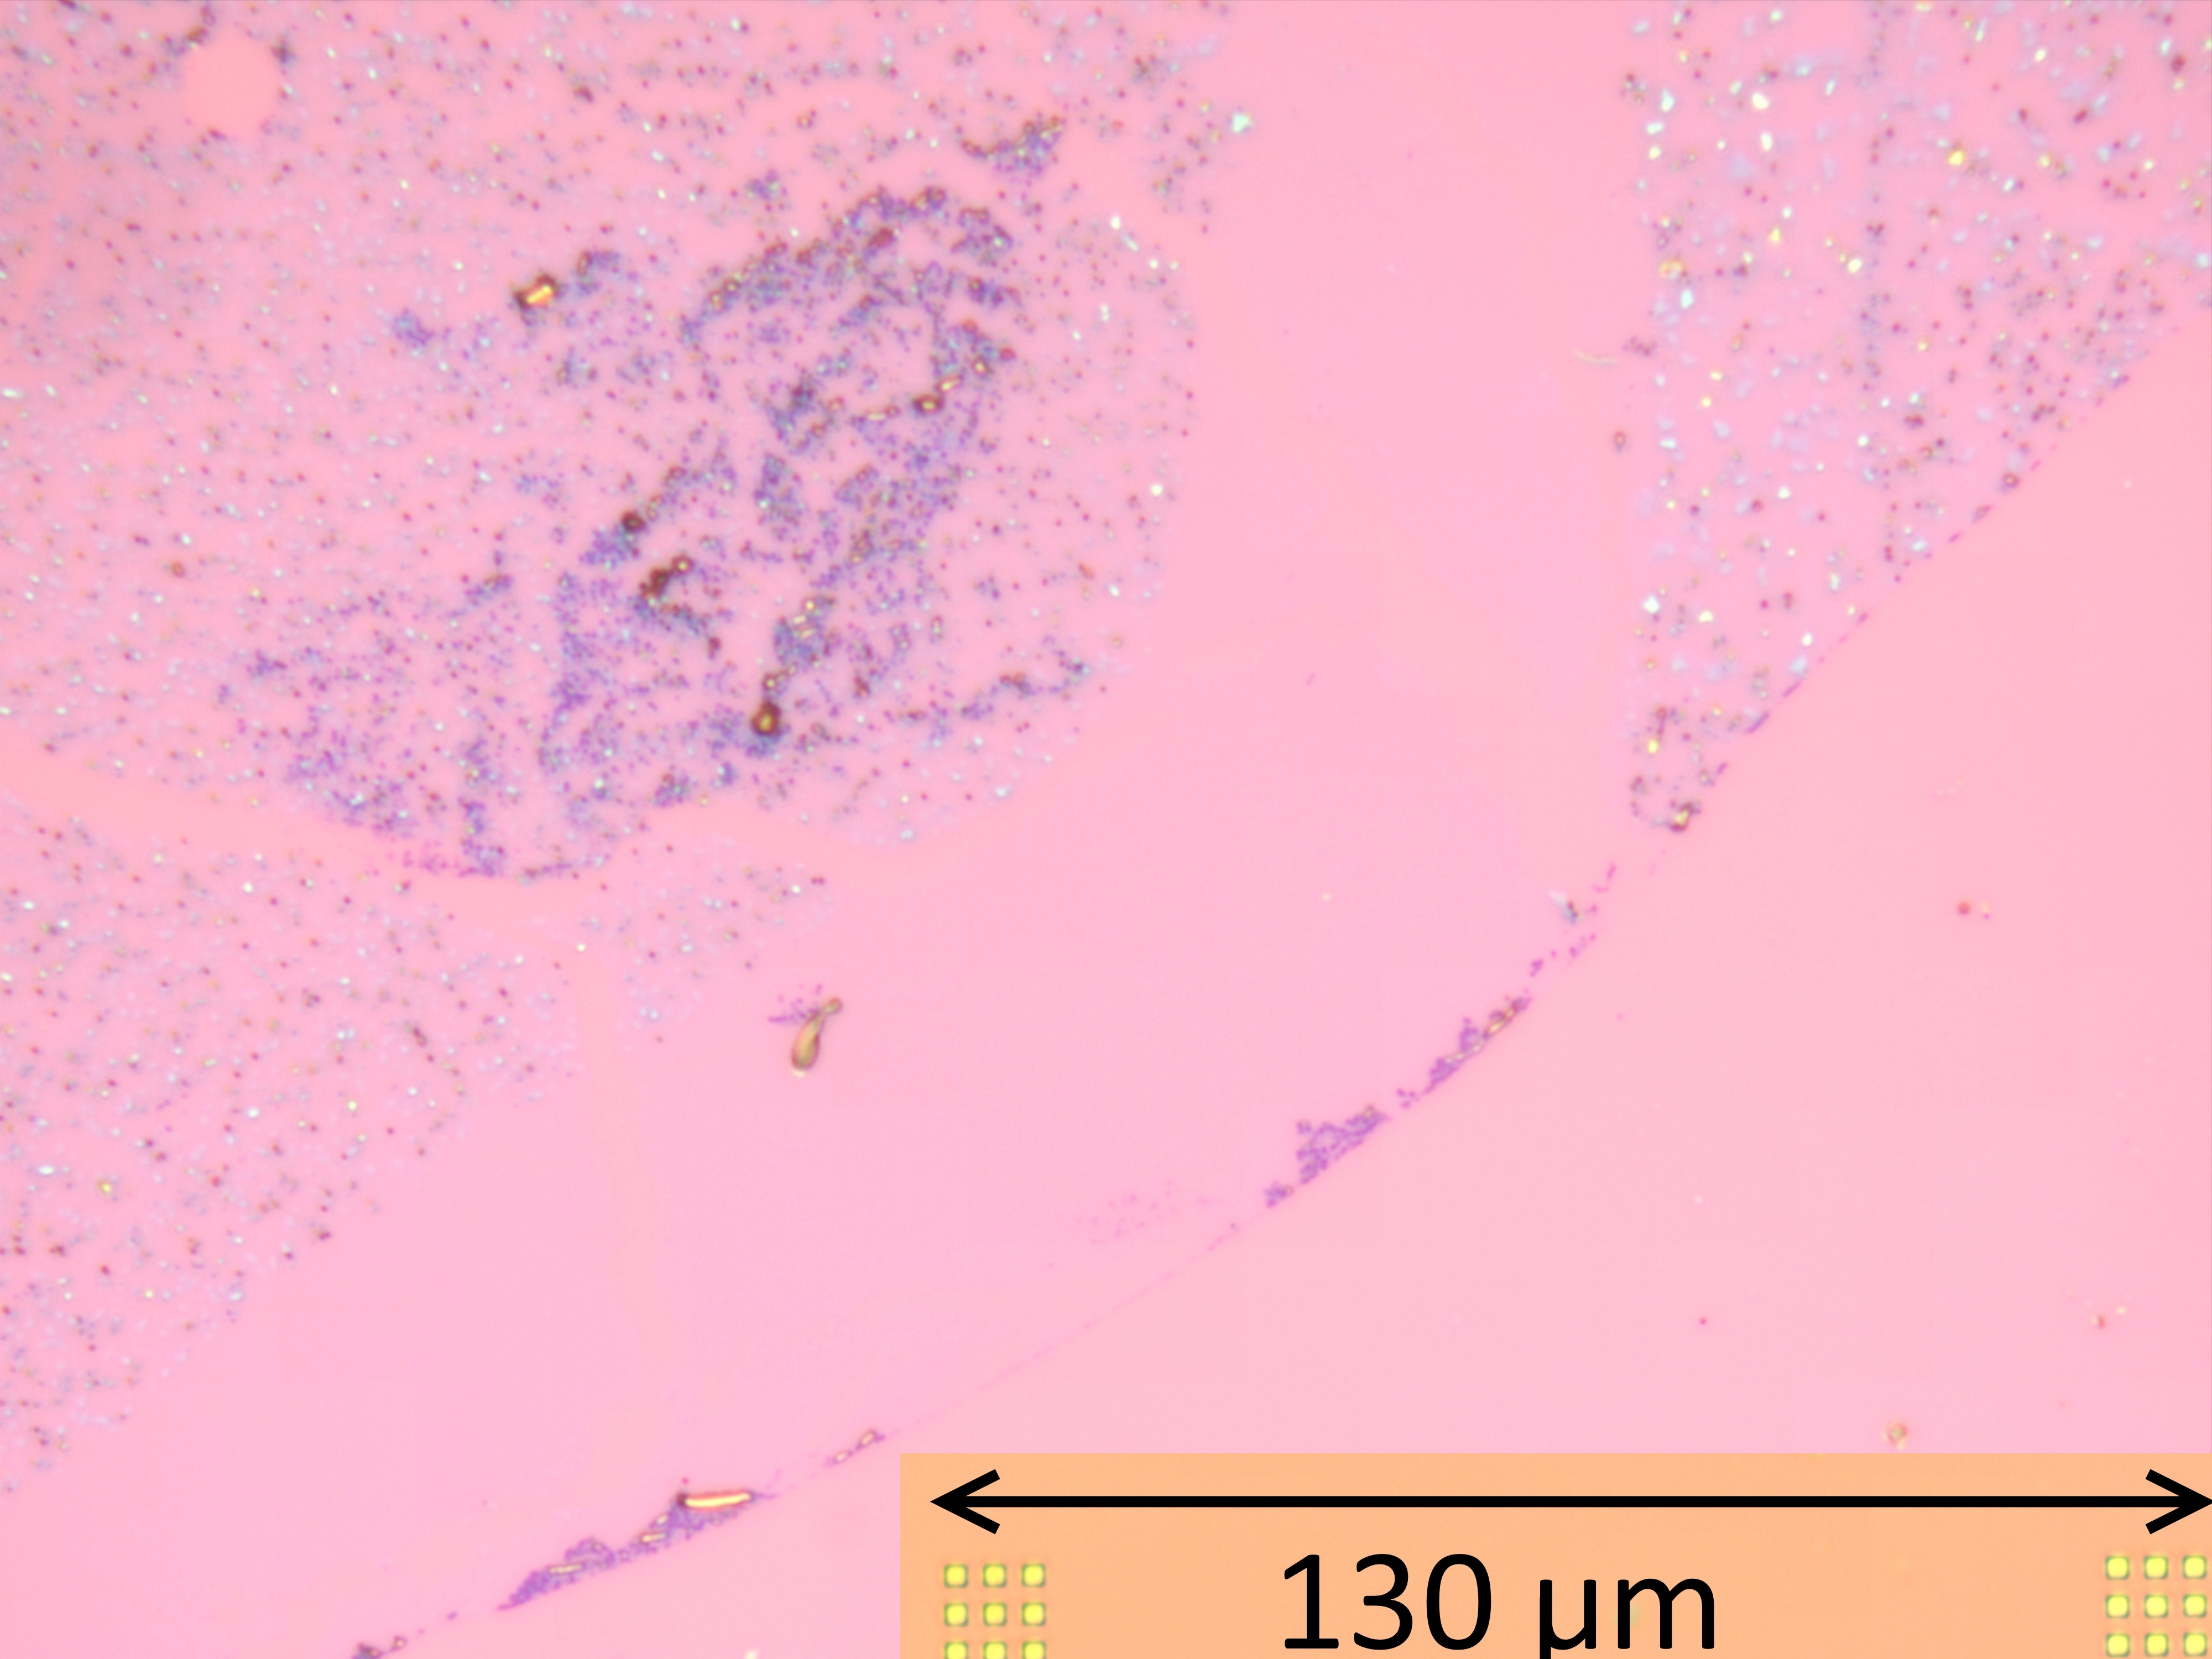
\includegraphics[width=0.95\textwidth,angle=0]{chap5/bi2o3/transfer2_50x}
			\caption{\bismuthoxide{} with nearby metal - 50x}\label{fig:bi2o3_4}
		\end{subfigure}
		\begin{subfigure}[t]{0.24\textwidth}
			\centering
			\includegraphics[width=0.95\textwidth,angle=0]{chap5/sno/transfer2}
			\caption{Clean \tinoxide{} sheet with some metal remnant}\label{fig:sno_3}
		\end{subfigure}
		\begin{subfigure}[t]{0.24\textwidth}
			\centering
			\includegraphics[width=0.95\textwidth,angle=0]{chap5/sno/transfer3}
			\caption{\tinoxide{} sheet with holes}\label{fig:sno_4}
		\end{subfigure}
		\caption[\bismuthoxide{} and \tinoxide{} printing on \silicondioxide{}]{Deposition of \bismuthoxide{} and \tinoxide{} onto \silicondioxide{}. Scale bar: 0.13mm}\label{fig:transfer_bi&sno_on_si}
	\end{figure}
	
	Sheets are much more uniform and easy to come by than that of \aluminimumoxide{}. Unfortunately it was still clear (\cref{fig:goldbismuthtin}) that, for both bismuth and tin metals, adhesion to gold contacts was still a significant problem and resulted in very little oxide transfer. This is likely due to the breaking of the thin oxides surface during contact and interaction thereafter of metals.
	\begin{figure}[H]
		\centering
		\begin{subfigure}[t]{0.19\textwidth}
			\includegraphics[width=\textwidth]{chap5/bi2o3/gtransfer1}
			\caption{Bismuth/gold interaction}\label{fig:goldbistin1}
		\end{subfigure}
		\begin{subfigure}[t]{0.19\textwidth}
			\includegraphics[width=\textwidth]{chap5/bi2o3/gtransfer2}			
			\caption{Bismuth removing gold and revealing chromium layer underneath}
		\end{subfigure}
		\begin{subfigure}[t]{0.19\textwidth}
			\includegraphics[width=\textwidth]{chap5/bi2o3/gtransfer3}
			\caption{Bismuth/gold interaction}
		\end{subfigure}
		\begin{subfigure}[t]{0.19\textwidth}
			\includegraphics[width=\textwidth]{chap5/bi2o3/gtransfer4}
			\caption{Bismuth removing areas of gold}
		\end{subfigure}
		\begin{subfigure}[t]{0.19\textwidth}
			\includegraphics[width=\textwidth]{chap5/sno/gtransfer1}
			\caption{Tin removing gold}
		\end{subfigure}\\
		\begin{subfigure}[t]{0.19\textwidth}
			\includegraphics[width=\textwidth]{chap5/sno/gtransfer2}
			\caption{Tin adhering to gold of device pads}
		\end{subfigure}
		\begin{subfigure}[t]{0.19\textwidth}
			\includegraphics[width=\textwidth]{chap5/sno/gtransfer3}
			\caption{Tin depositing some small oxide}
		\end{subfigure}
		\begin{subfigure}[t]{0.19\textwidth}
			\includegraphics[width=\textwidth]{chap5/sno/gtransfer4}
			\caption{Tin removing large area gold}
		\end{subfigure}
		\begin{subfigure}[t]{0.19\textwidth}
			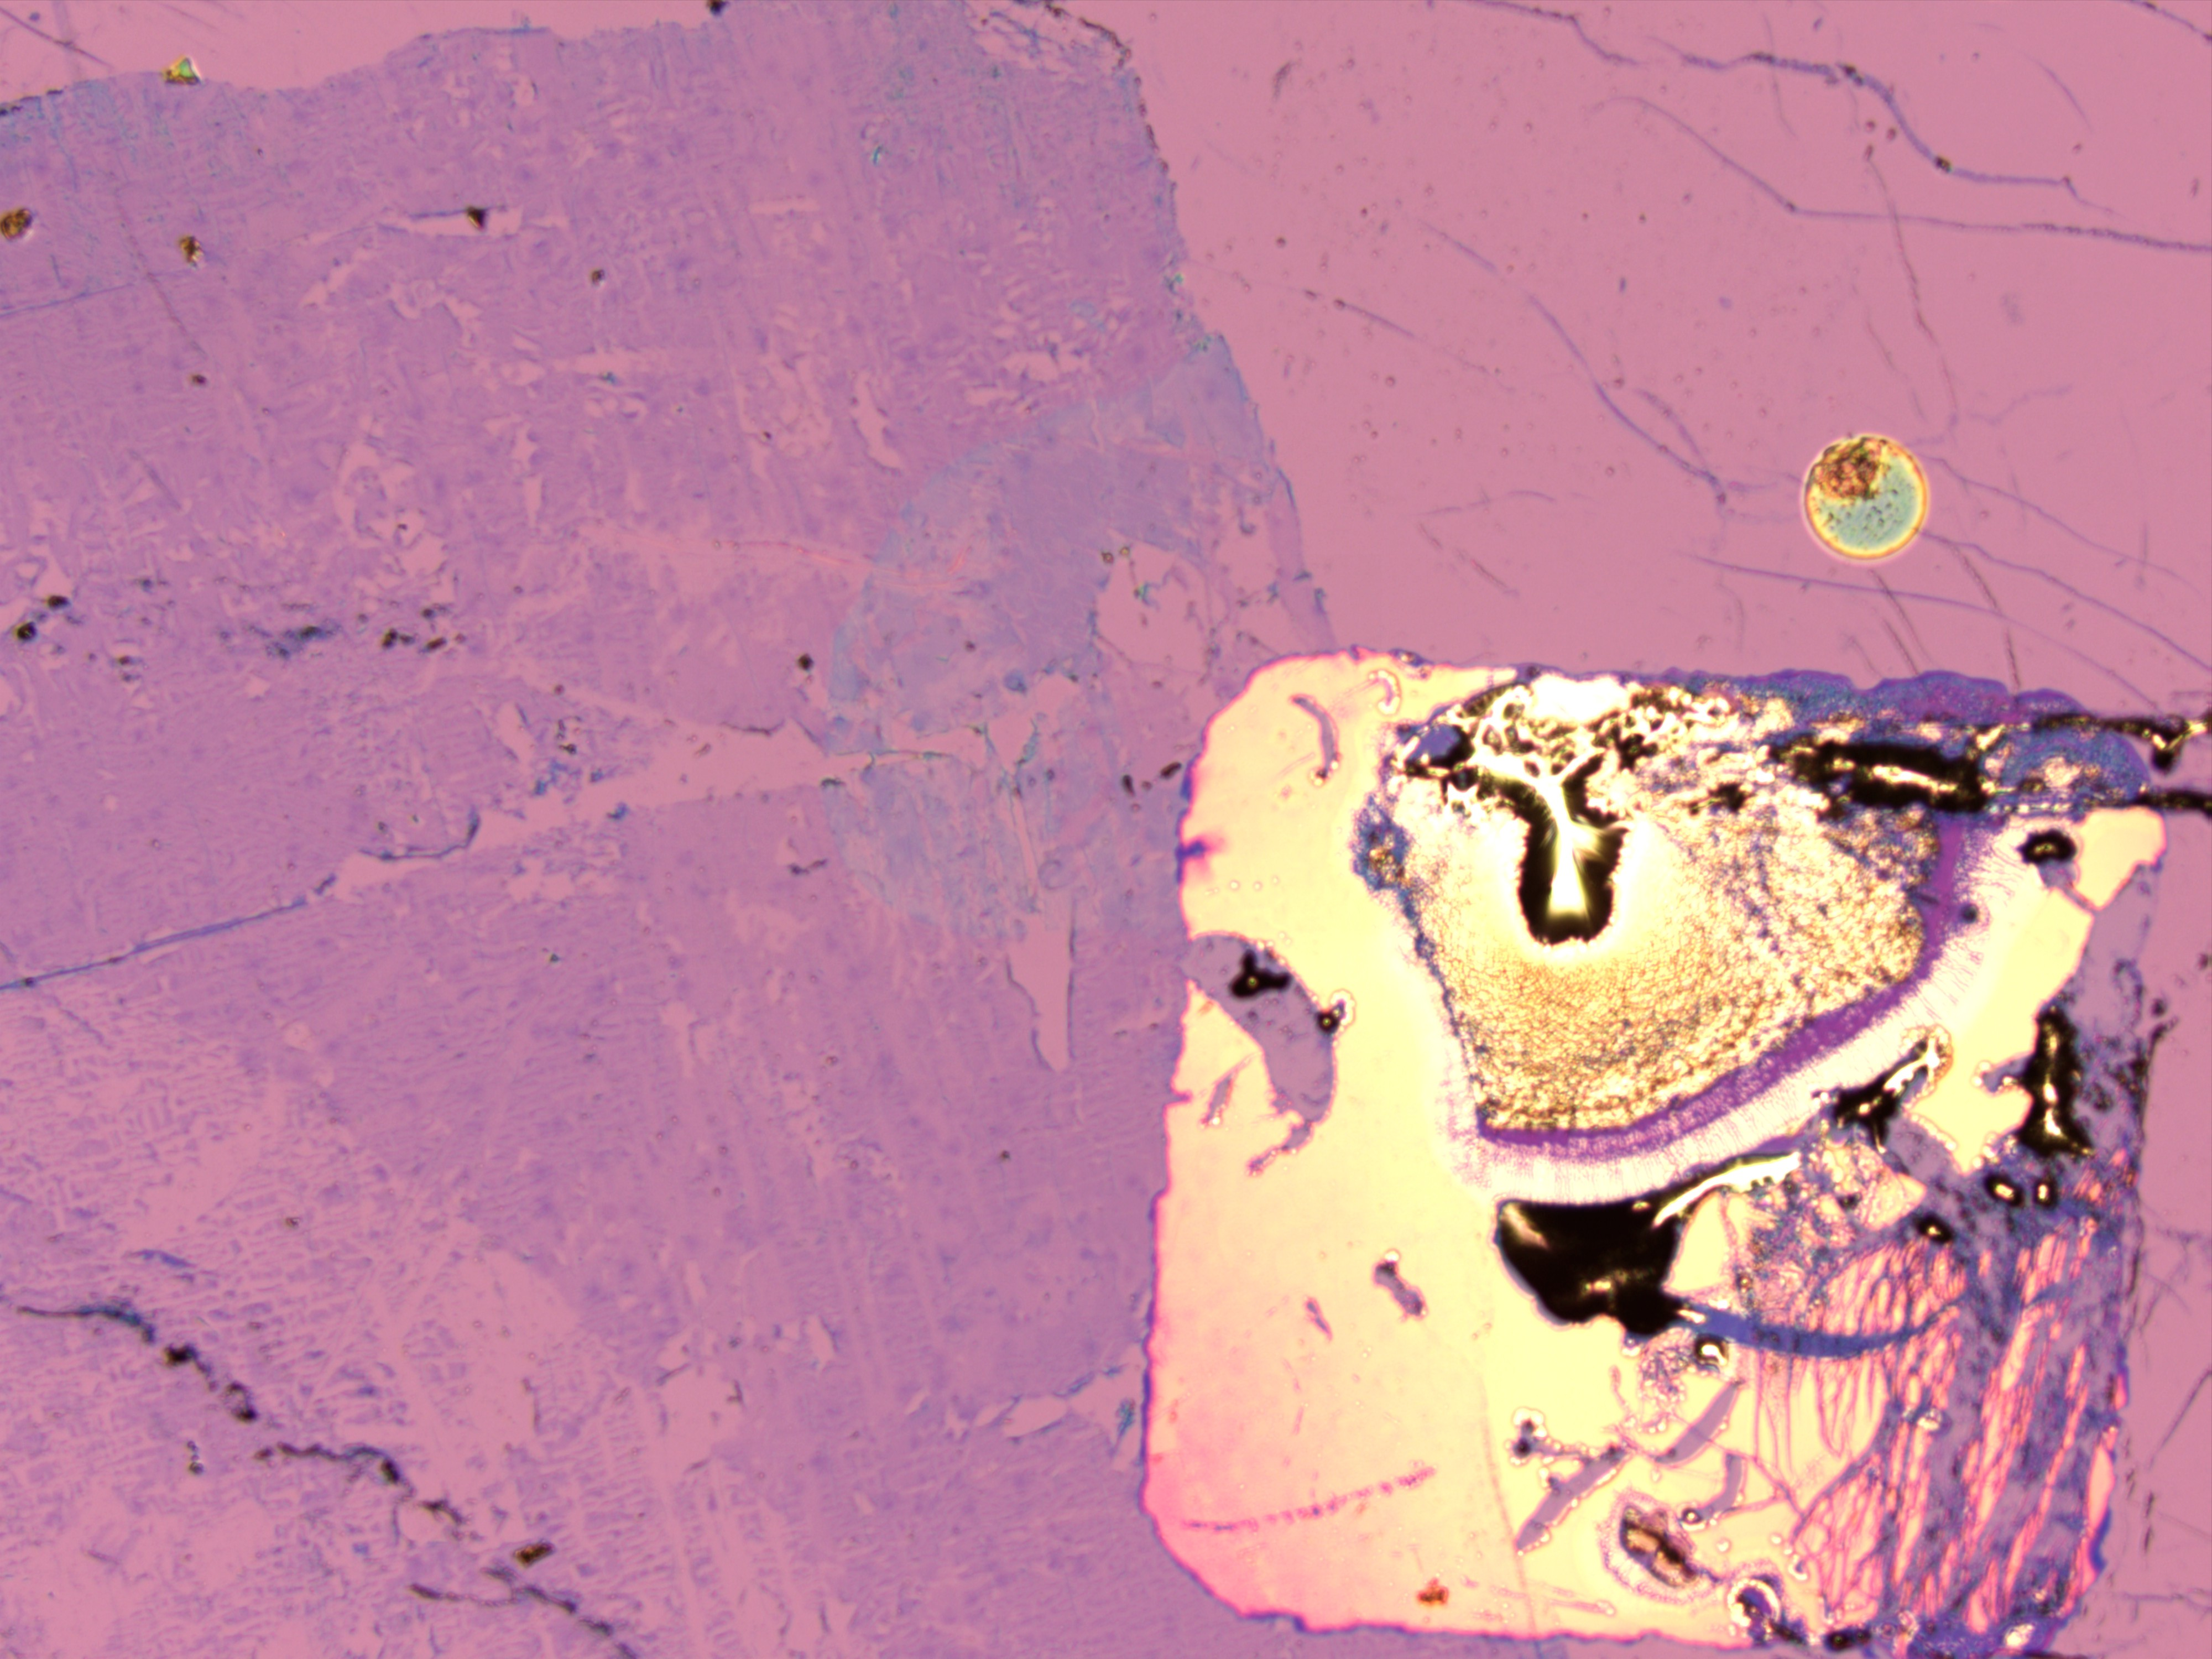
\includegraphics[width=\textwidth]{chap5/sno/gtransfer5}
			\caption{Tin not interacting with CVD graphene, but adhering to gold pad.}
		\end{subfigure}
		\begin{subfigure}[t]{0.19\textwidth}
			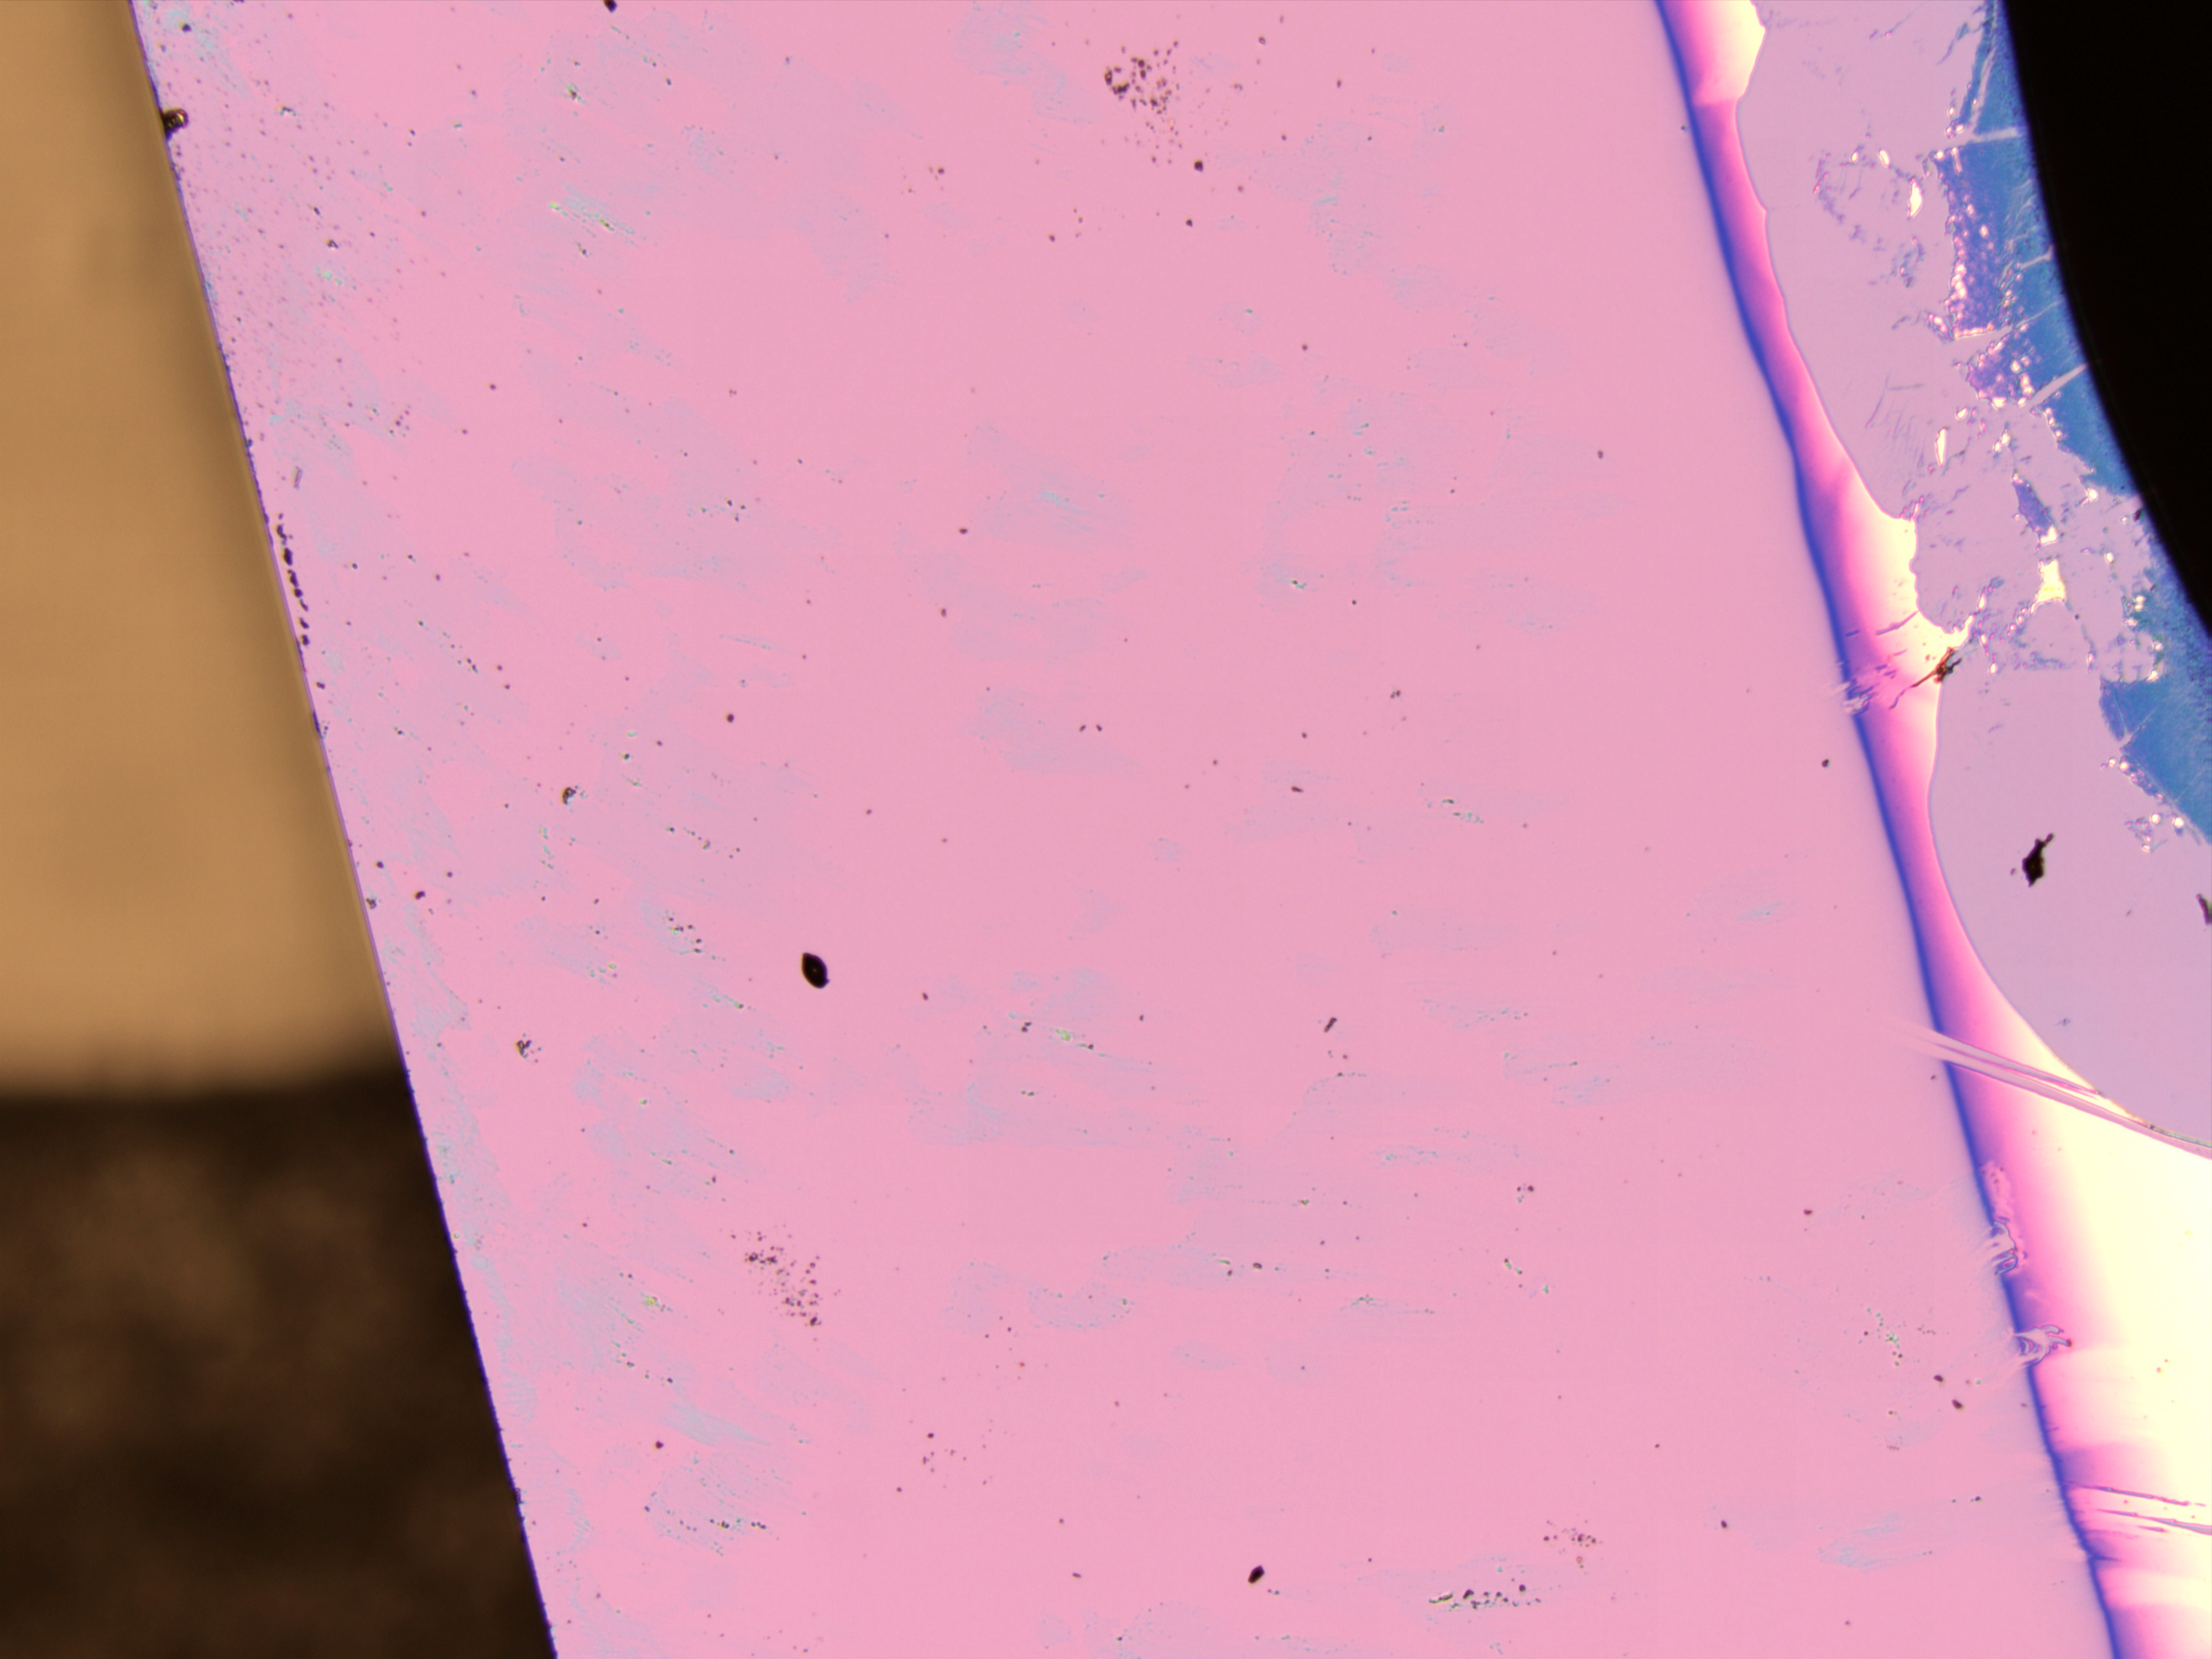
\includegraphics[width=\textwidth]{chap5/sno/gtransfer6}
			\caption{\tinoxide{} with gold removal.}
		\end{subfigure}
		\caption[Strong gold bismuth/tin interaction]{Strong gold bismuth/tin interaction. All images with same scalebar as \cref{fig:goldbistin1}, 130 $\mu$m.}\label{fig:goldbismuthtin}
	\end{figure}
	
	To reduce this gold-liquid metal reaction occuring across gallium, bismuth and tin, we (my supervisors \& Torben) concluded we had a few options to proceed. Firstly, other metals could be used to make conduction pads such as tungsten, which would react less with the liquid metals. Secondly the possibility of a different approach such as transferring oxides onto \silicondioxide{} and then attempting some transfer of graphene, like with CVD. 
	
	Thirdly, we could try to add layers of protection above the gold to create distance from the liquid metal. An issue with this method is that for thin oxides, creating high 2D lithography structures begins to create bends/steps in any oxide deposition possibly reducing the chance of a successful transfer.
	
	We decided to attempt using extra deposition layers to protect our gold contact pads, because transferring would take some time and have slow throughput, and gold was quite preferential due to it's conductive properties and use in the probestation. We also decided to focus on gallium and tin, due to their reliability and uniformity over bismuth.
	
	The first protective layer used followed a combination of 2nm Cr $\vert$ 50nm Au $\vert$ 2nm Cr $\vert$ 10nm \silicondioxide{}. Clear improvements were seen in success of the deposition of gallium oxide, as will be shown in \cref{sec:smearing}. Tin also showed improvements, however the liquid-metal gold interaction was still strong enough to cause damager (smaller than previous) to the contact pads, suggesting a larger layer protective \silicondioxide{} was required.
	
	This led us to our final protection thickness of 20nm of \silicondioxide{} deposited on top of our gold contact pads, in which we have had successful transfers with \galliumoxide{}, however haven't been able to test \tinoxide{} transfers again due to time constraints.
	
	\section{Smearing Ga$_2$O$_3$}\label{sec:smearing}
	At RMIT, I was also introduced to a slightly different method of depositing thin oxides, from Nitu. This technique is shown in detail  in \cref{fig:gallium_transfer_process}, and involves the rolling or smearing of a liquid metal droplet between two substrates.
	\begin{figure}[H]
		\begin{subfigure}{0.24\textwidth}
			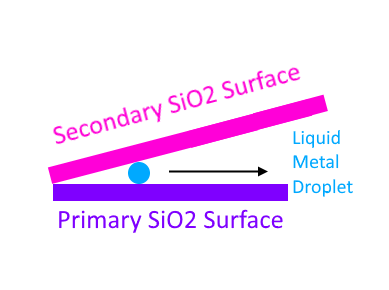
\includegraphics[width=\textwidth]{chap5/ga2o3/proc1}
			\caption{Liquid metal droplet placed directly between \silicondioxide{} wafers}
		\end{subfigure}
		\begin{subfigure}{0.24\textwidth}
			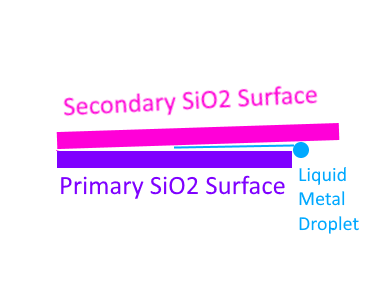
\includegraphics[width=\textwidth]{chap5/ga2o3/proc2}
			\caption{Liquid metal droplet smeared by pressing \silicondioxide{} together in a directional action}
		\end{subfigure}
		\begin{subfigure}{0.24\textwidth}
			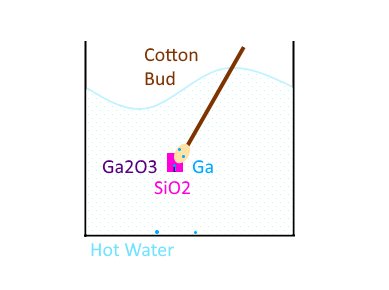
\includegraphics[width=\textwidth]{chap5/ga2o3/proc3}
			\caption{Cleaning of remaining gallium metal in 100 $^\circ$C water with cotton buds}
		\end{subfigure}
		\begin{subfigure}{0.24\textwidth}
			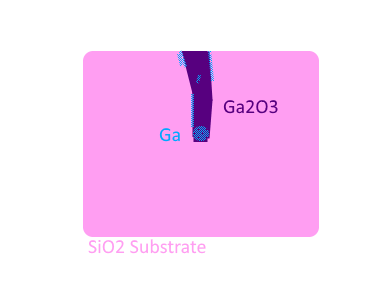
\includegraphics[width=\textwidth]{chap5/ga2o3/proc4}
			\caption{Remaining \galliumoxide{} with some gallium metal residues}
		\end{subfigure}
		\caption[\galliumoxide{} transfer process]{\galliumoxide{} transfer process}\label{fig:gallium_transfer_process}
	\end{figure}
	A step of cleaning is required to remove as much remaining oxide as possible, and this is done by placing the substrate into a beaker of hot water ($\approx 100$ $^\circ$C) where the liquid metal is hydrophobic to the water, returns to a ball geometry allowing clean removal of large clumps with a cotton bud (adhesive to liquid gallium). Unfortunately the use of the cotton bud can also result in scratching of the gallium oxide and hence requires care when dabbing/rubbing the metal contaminated regions.
	
	Initially without oxide protection for gold, we observe (\cref{fig:smear1}) very similar results to that of \bismuthoxide{} and \tinoxide{}, with large sheet deposition, perhaps with a little less uniformity. Deposition onto gold pads was more successful that other methods in that significant amounts of oxide were deposited, however interaction with pads was very damaging.
	\begin{figure}[H]
		\begin{subfigure}[t]{0.24\textwidth}
			\includegraphics[width=\textwidth]{chap5/ga2o3/transfer1}
			\caption{Large sheets of \galliumoxide{}}\label{fig:smear1a}
		\end{subfigure}
		\begin{subfigure}[t]{0.24\textwidth}
			\includegraphics[width=\textwidth]{chap5/ga2o3/transfer2}
			\caption{\galliumoxide{} of varying thicknesses}
		\end{subfigure}
		\begin{subfigure}[t]{0.24\textwidth}
			\includegraphics[width=\textwidth]{chap5/ga2o3/transfer3}
			\caption{\galliumoxide{} prior to cleaning}
		\end{subfigure}
		\begin{subfigure}[t]{0.24\textwidth}
			\includegraphics[width=\textwidth]{chap5/ga2o3/transfer4}
			\caption{\galliumoxide{} prior to cleaning with significant metal contamination}
		\end{subfigure}\\
		\begin{subfigure}[t]{0.24\textwidth}
			\includegraphics[width=\textwidth]{chap5/ga2o3/gtransfer1}
			\caption{Gallium \& gold interaction with \galliumoxide{} deposition}
		\end{subfigure}
		\begin{subfigure}[t]{0.24\textwidth}
			\includegraphics[width=\textwidth]{chap5/ga2o3/gtransfer2}
			\caption{Localised \galliumoxide{} deposition at gold edge}
		\end{subfigure}
		\begin{subfigure}[t]{0.24\textwidth}
			\includegraphics[width=\textwidth]{chap5/ga2o3/gtransfer3}
			\caption{Strong gallium \& gold interaction}
		\end{subfigure}
		\begin{subfigure}[t]{0.24\textwidth}
			\includegraphics[width=\textwidth]{chap5/ga2o3/gtransfer4}
			\caption{Strong gallium \& gold interaction}
		\end{subfigure}
		\caption[Smearing of \galliumoxide{} on CVD graphene, Au and \silicondioxide{}]{Smearing of \galliumoxide{} on CVD graphene, Au and \silicondioxide{}. Scale is uniform across all images, the same as \cref{fig:smear1a}, 130 $\mu$m.}\label{fig:smear1}
	\end{figure}
	An attempt at applying \galliumoxide{} onto CVD graphene turned out to completely destroy the layer of graphene, likely during the cleaning process (\cref{fig:ga_cvd}). Given the size of the oxides being able to be deposited onto gold pads at this point, we did not try to deposit on top of CVD graphene any further in the knowledge that a small exfoliated device would likely have larger success, and is preferential for it's transport characteristics.

	\begin{figure}[H]
		\begin{subfigure}{0.5\textwidth}
			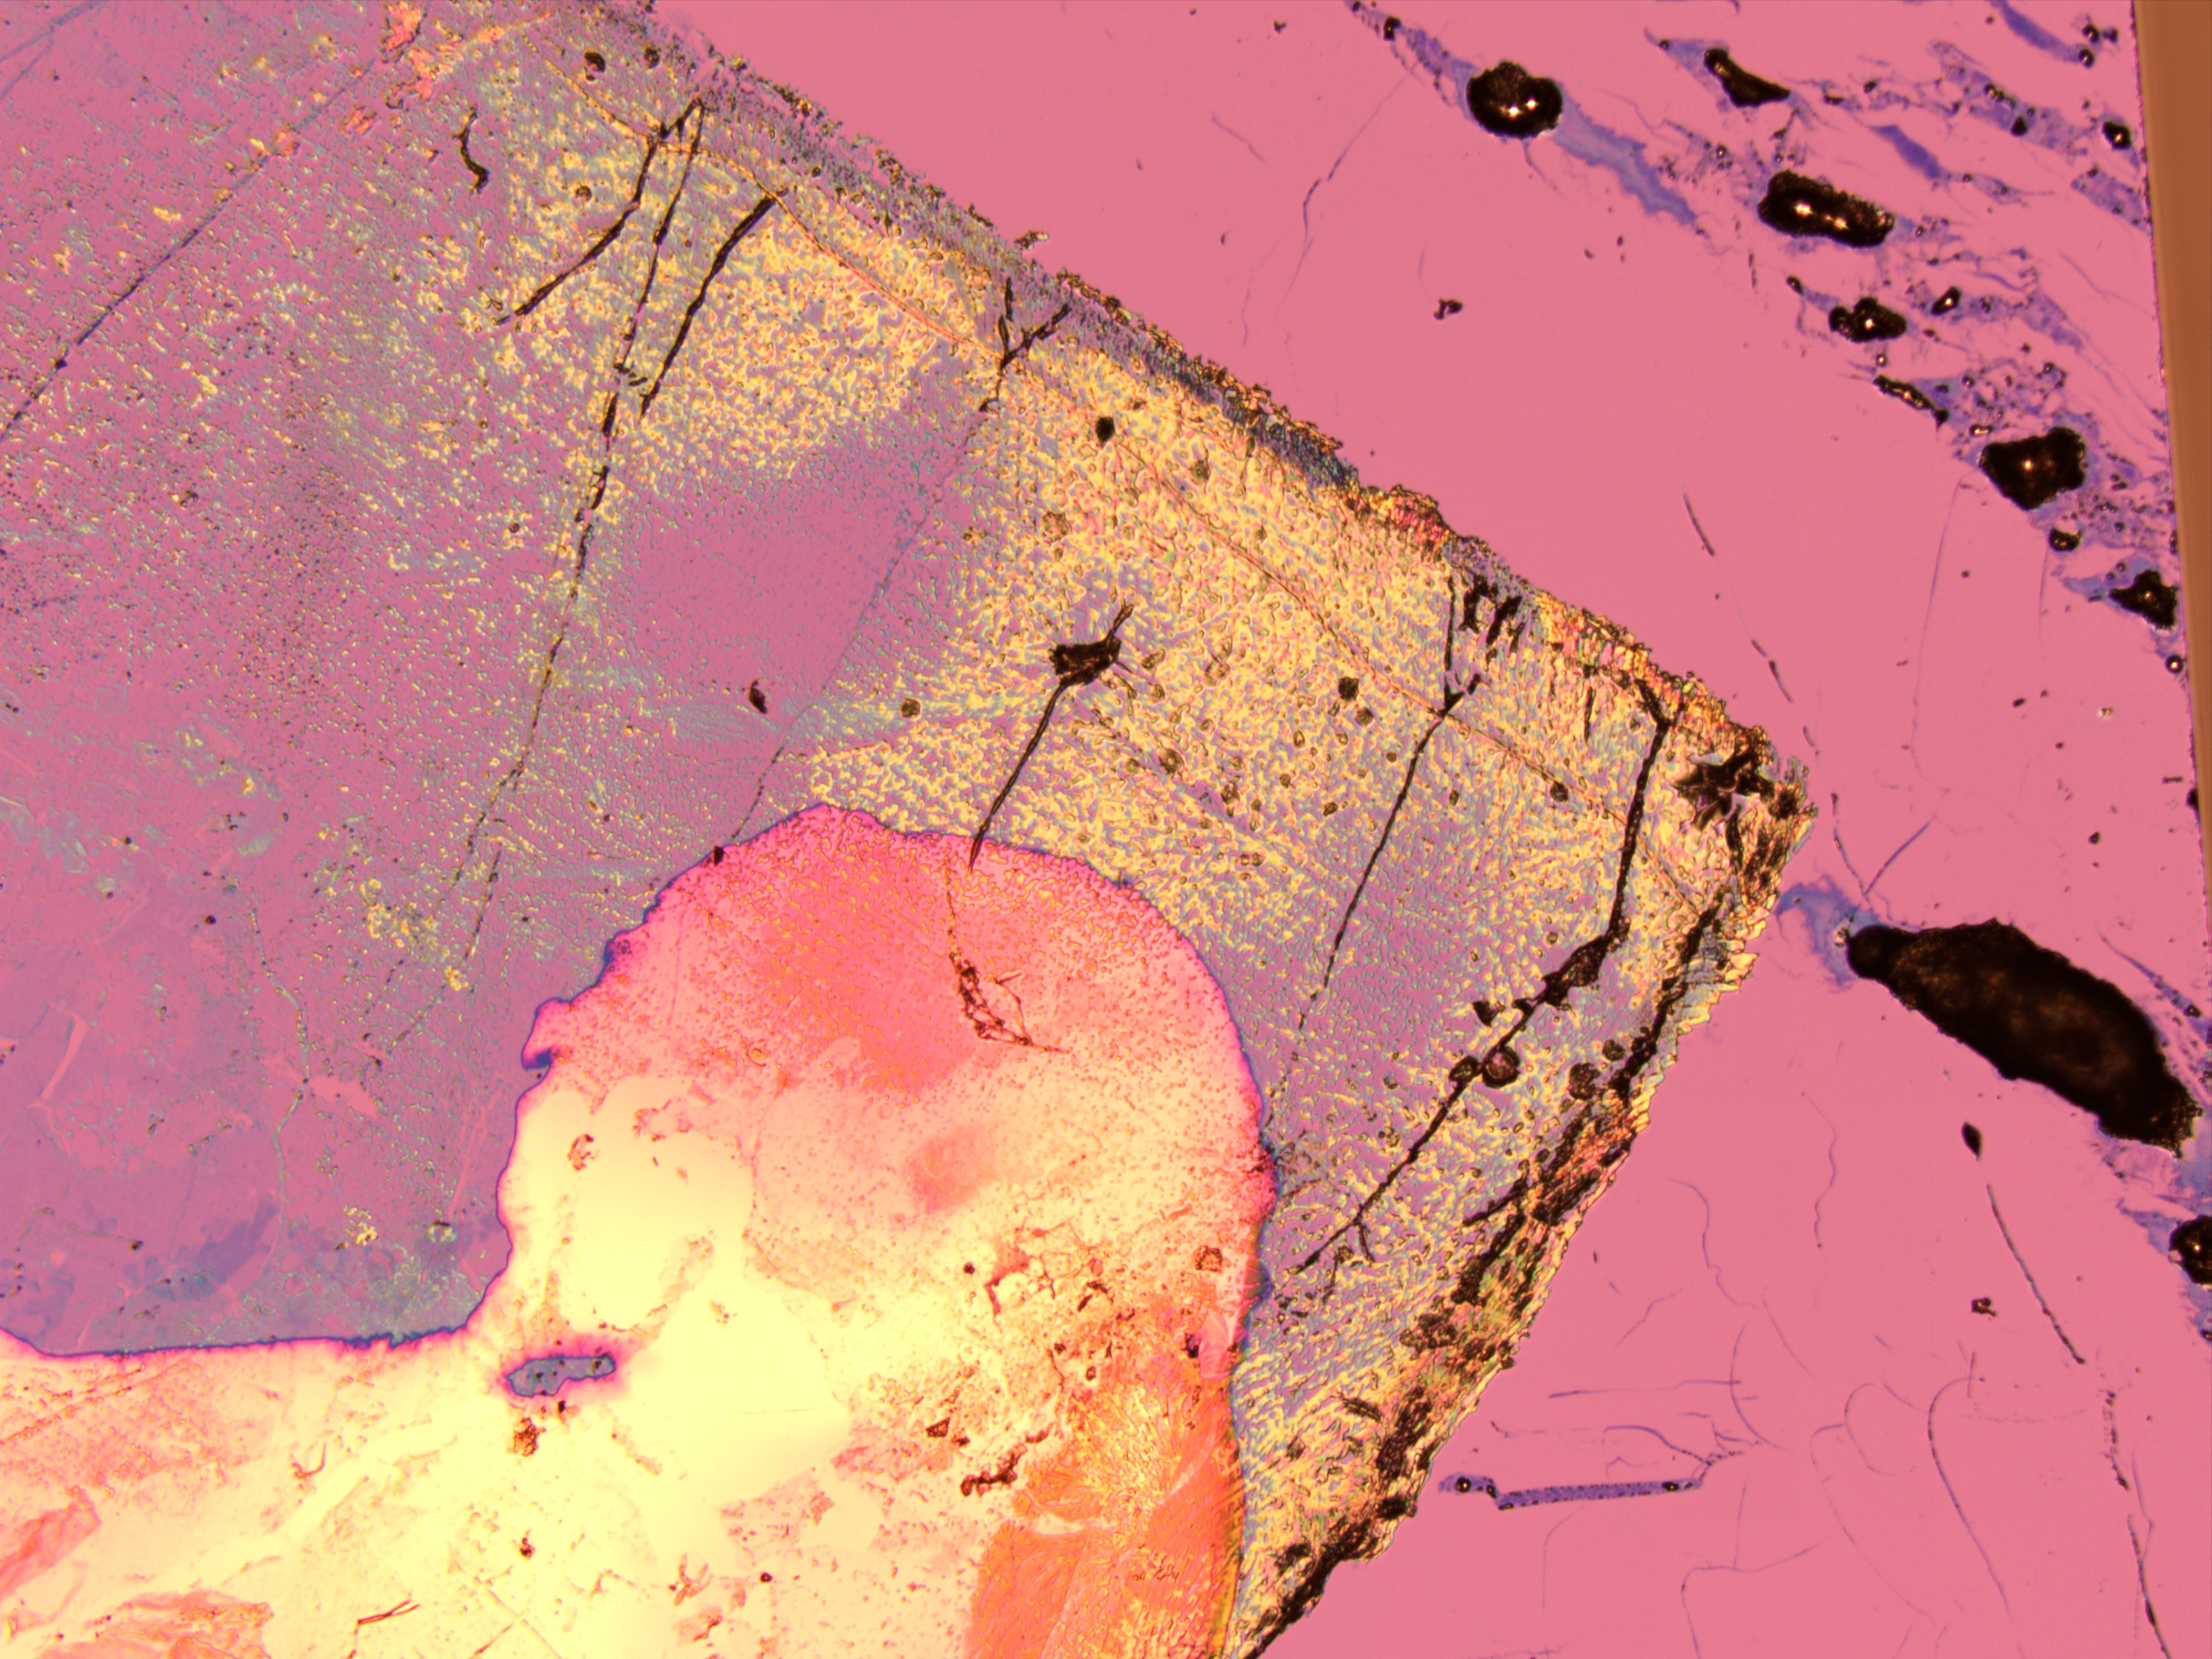
\includegraphics[width=0.8\textwidth]{chap5/ga2o3/ctransfer_before}
			\caption{Before}
		\end{subfigure}
		\begin{subfigure}{0.5\textwidth}
			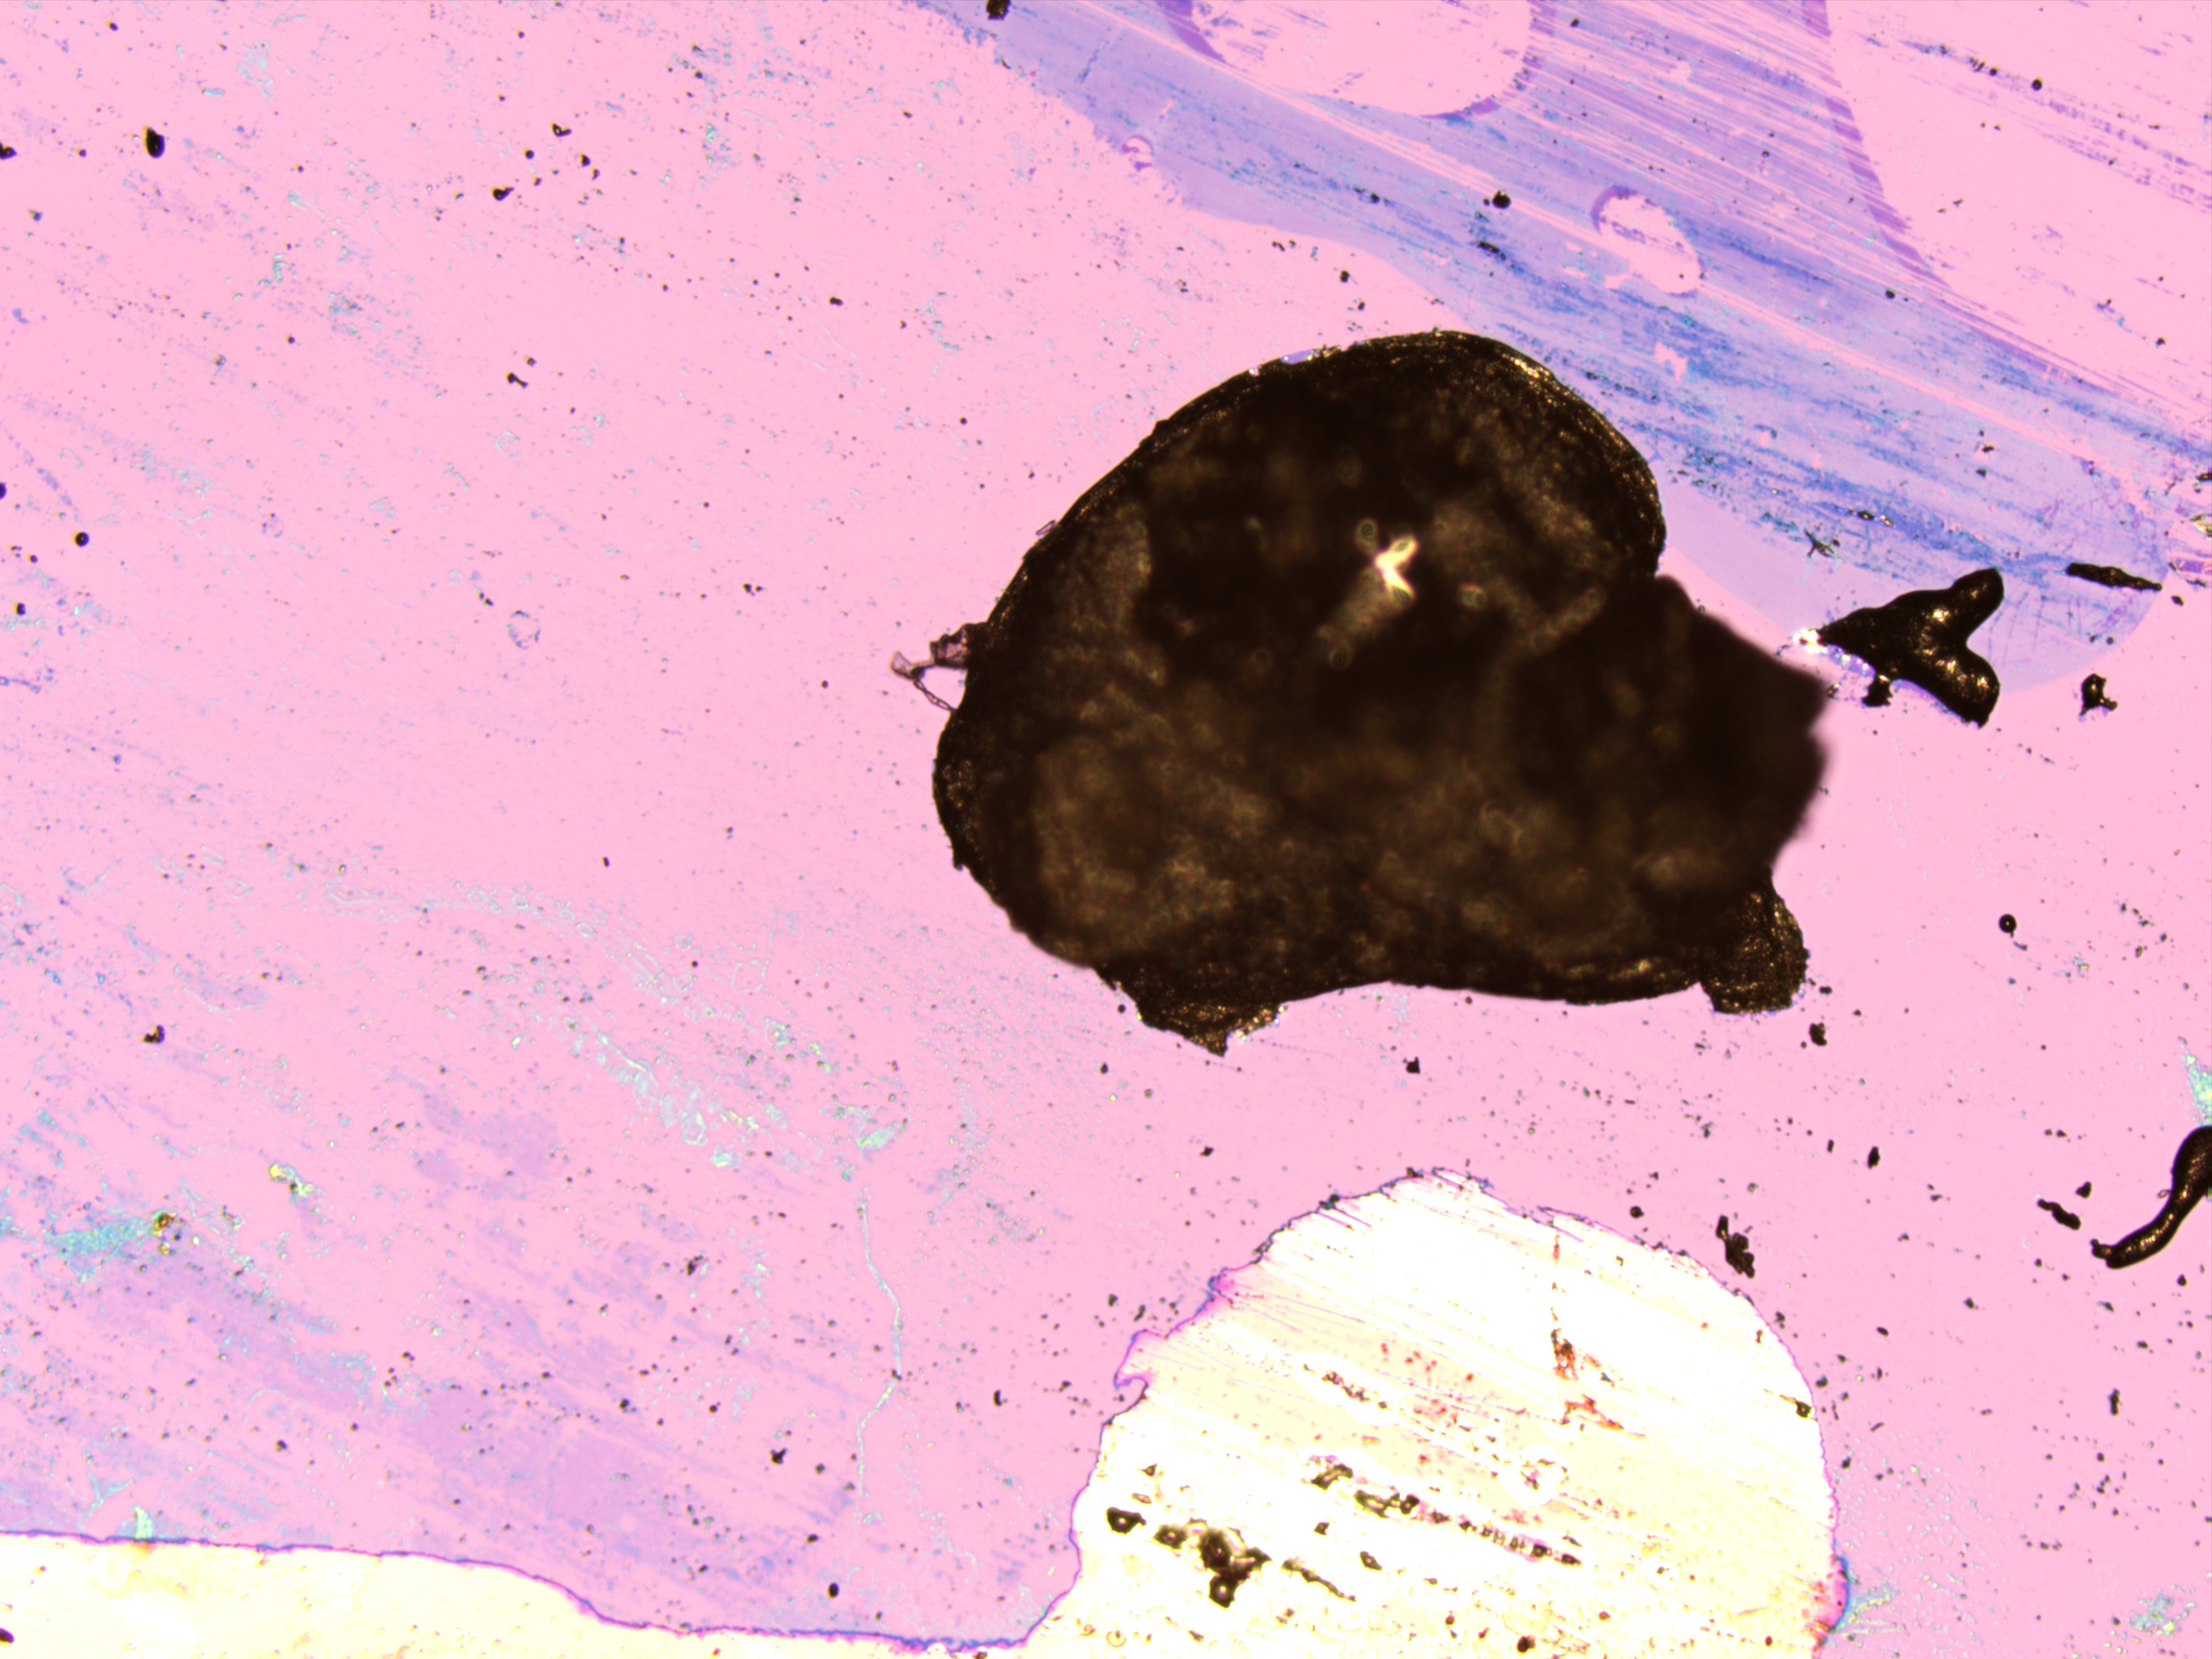
\includegraphics[width=0.8\textwidth]{chap5/ga2o3/ctransfer_after}
			\caption{After}
		\end{subfigure}
		\caption{Attempted smearing of \galliumoxide{} onto CVD graphene}\label{fig:ga_cvd}
	\end{figure}

	After applying a 10nm protection layer, we achieved our first fake device coverages on fine gold pads, shown in .
	\begin{figure}[H]
		\begin{subfigure}{}
			content...
		\end{subfigure}
		\caption[Smearing of \galliumoxide{} with 10nm \silicondioxide{} protection layer]{}\label{fig:smear2}
	\end{figure}
	
	At this point I returned from RMIT with a vial of gallium metal to be able to futher conduct printing trials at Monash.
	
	\begin{figure}[H]
		\caption[Smearing of \galliumoxide{} with 20nm \silicondioxide{} protection layer]{}
	\end{figure}
	
	\subsection{Devices}
	
	
	

\end{document}